\chapter{Robots Móviles y Agentes Inteligentes}


\section{Máquina de Estado}

\begin{itemize}
	\item[\textbullet] Entradas
	\item[\textbullet] Máquinas
	\item[\textbullet] Salidas
\end{itemize}

\section{Máquina de Estado Aumentada}

Una entrada (o salida) de una máquina puede ser sustituida por la salida de otra máquina de estados. Esa bloquea la entrada (o salida) ordinaria y pone su salida.

\begin{figure}[h!]
	\centering
	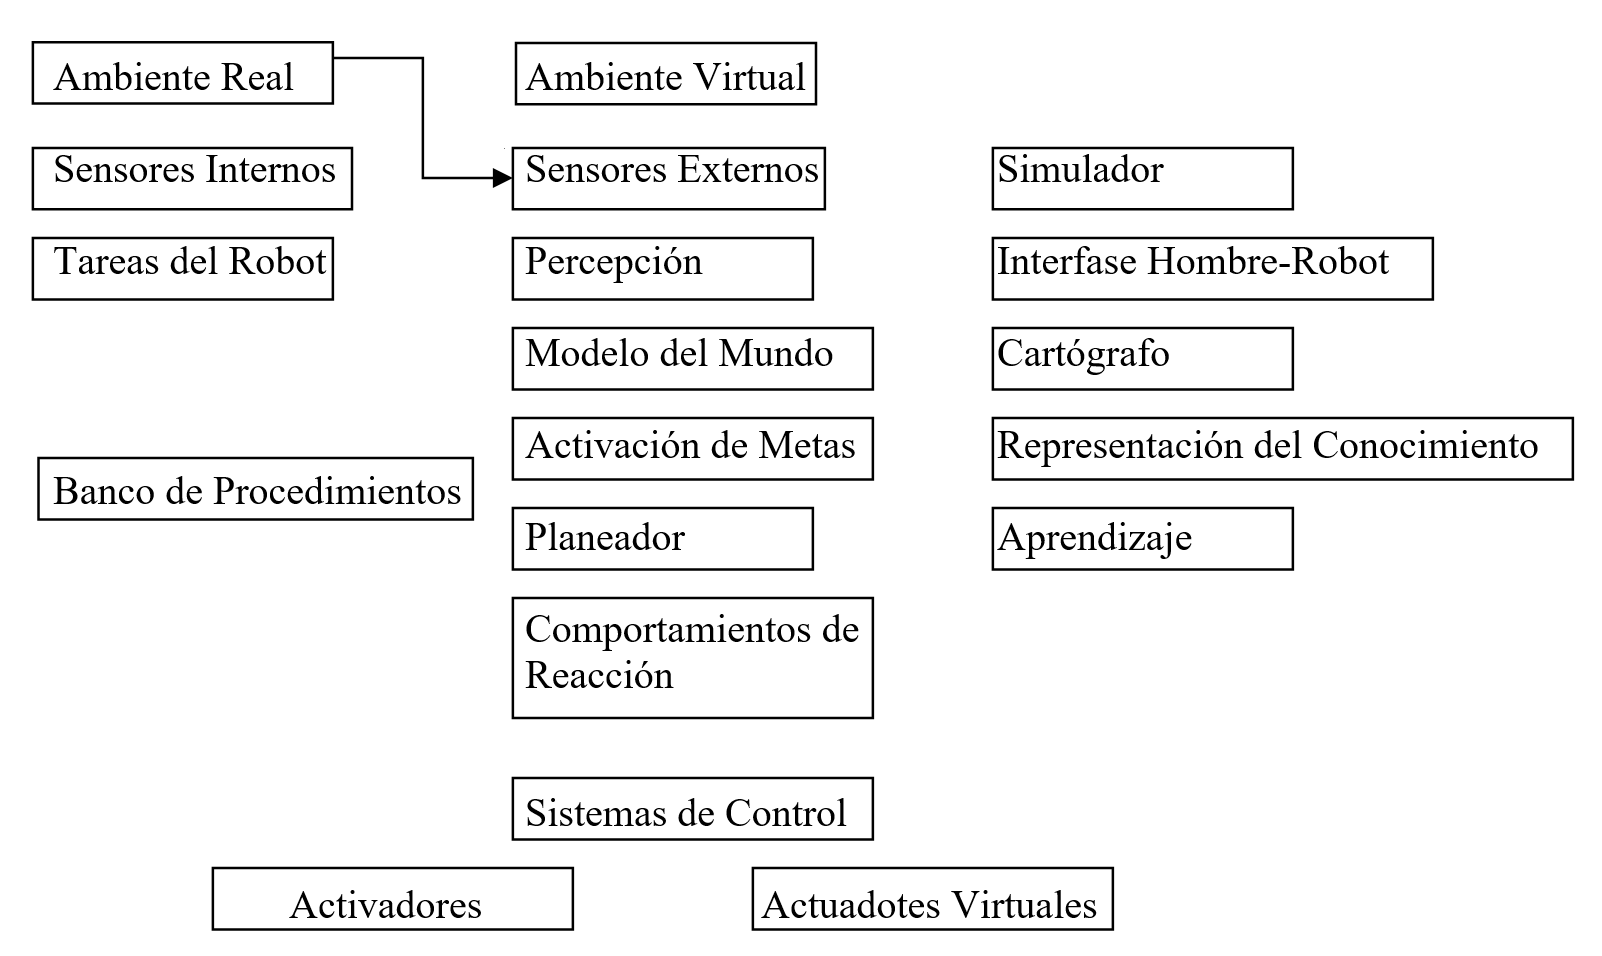
\includegraphics[width=0.5\textwidth]{images/img49.png}
	\label{figura49}
\end{figure}

\section{Arquitecturas Reactivas (o por Comportamientos)}

Diagramas de Stimulus Response (SR)

\begin{figure}[h!]
	\centering
	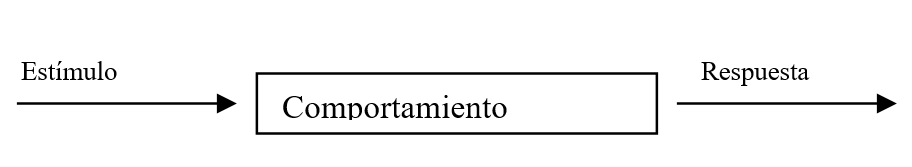
\includegraphics[width=0.5\textwidth]{images/img50.png}
	\label{figura50}
\end{figure}

La idea es que la respuesta sea instantánea.
En los comportamientos puros, la respuesta únicamente depende del estímulo.

\subsection{Organización de los comportamientos:} 

\textit{Esquema 1}

\begin{figure}[h!]
	\centering
	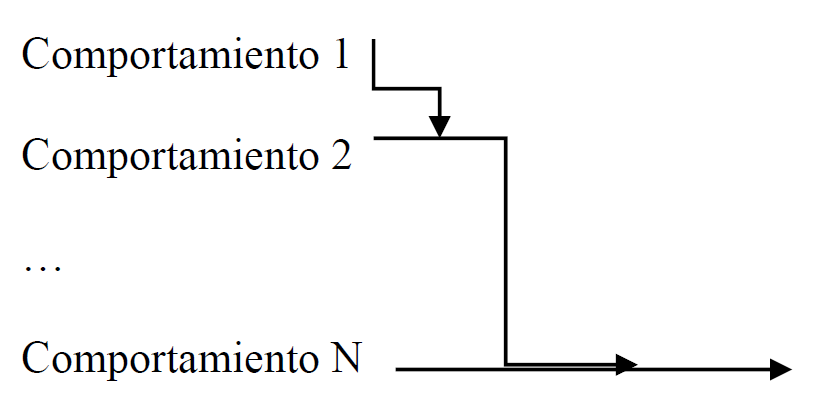
\includegraphics[width=0.5\textwidth]{images/img51.png}
	\label{figura51}
\end{figure}


Algunos comportamientos bloquean la salida de otros. Solamente la salida de uno es el que se usa, todos se activan. El diagrama anterior decide la prioridad.

La salida generalmente es un vector que, por ejemplo, indica la magnitud y dirección del movimiento del robot.

\textit{Esquema 2}

\begin{figure}[h!]
	\centering
	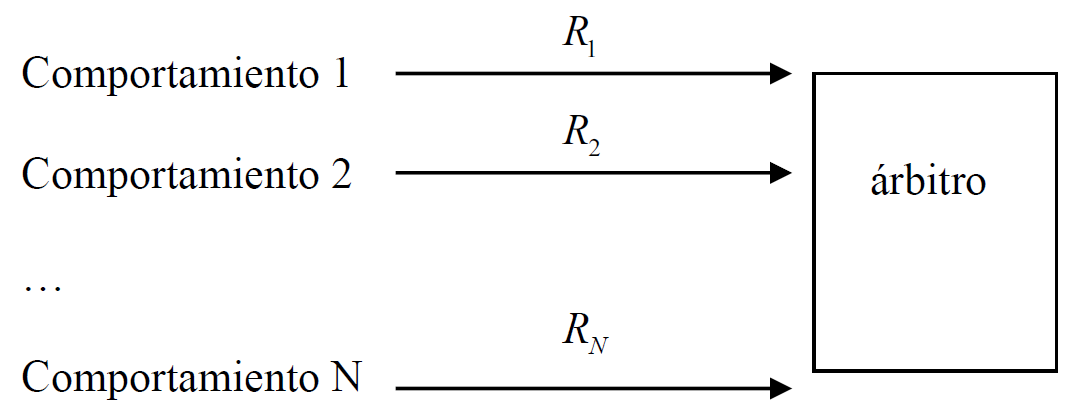
\includegraphics[width=0.5\textwidth]{images/img52.png}
	\label{figura52}
\end{figure}


El árbitro decide cuál es la respuesta.

\begin{figure}[h!]
	\centering
	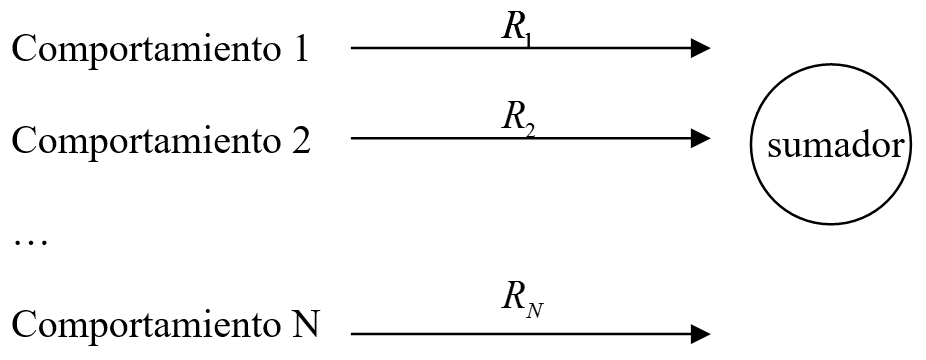
\includegraphics[width=0.5\textwidth]{images/img53.png}
	\label{figura53}
\end{figure}


El sumador hace un promedio ponderado por\textit{ganancias}.

$$
\sum_{i=1}^{N} \, g_i \, R_i
$$

La ganancia depende del diseñador y va a hacer que el robot se comporte de diferente forma (robot “audaz” contra robot “conservador”).

Un diagrama del espacio se puede hacer con campos vectoriales (diagramas de flechitas tipo sistemas dinámicos), por ejemplo uno que sea de las fuerzas de atracción y otro de repulsión y sumarlos.

Puedo tener una complejidad grande combinando comportamientos, pues pueden controlar diferentes cosas.


\section{Máquinas de Estado}
\subsection{Algoritmo para el Comportamiento de Evadir Obstáculos}

Un robot circula con:

\begin{itemize}
	\item[\textbullet] Dos motores, uno a cada lado.
	\item[\textbullet] Dos sensores adelante, para detectar obstáculos (por ejemplo, infrarrojos, ultrasonido, etc.)
\end{itemize}

\begin{figure}[h!]
	\centering
	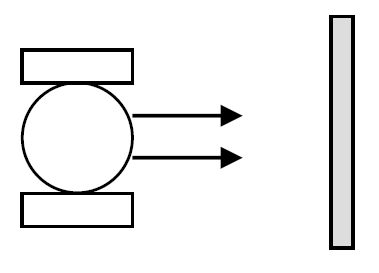
\includegraphics[width=0.5\textwidth]{images/img54.png}
	\label{figura54}
\end{figure}

Obviamente:
\begin{itemize}
	\item[\textbullet] Si los sensores no detectan el obstáculo, seguir 		avanzando.
	\item[\textbullet] Si el sensor derecho lo detecta y el otro no, hacerlo tantito para atrás y girar hacia la izquierda para seguir avanzando
	\item[\textbullet]Si el sensor izquierdo lo detecta y el otro no, hacerlo tantito para atrás y girar hacia la derecha para seguir avanzando
	\item[\textbullet]Si los dos detectan, hacerlo para atrás y giro 90°.
\end{itemize}

\begin{figure}[h!]
	\centering
	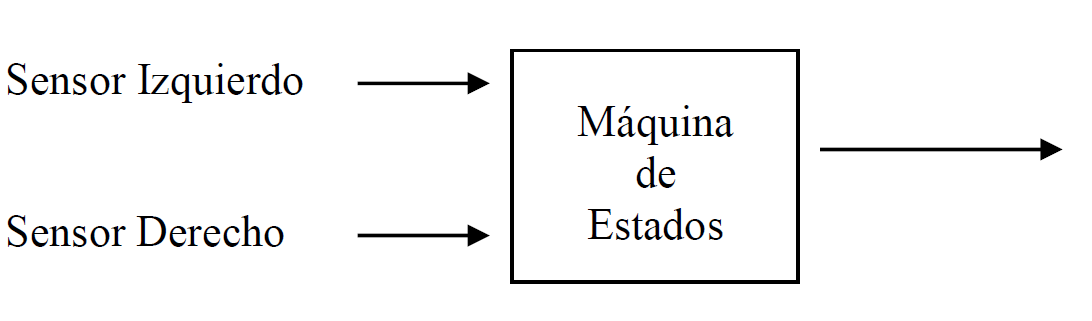
\includegraphics[width=0.5\textwidth]{images/img55.png}
	\label{figura55}
\end{figure}


\textit{Notación de diagrama de flujo}


\begin{figure}[h!]
	\centering
	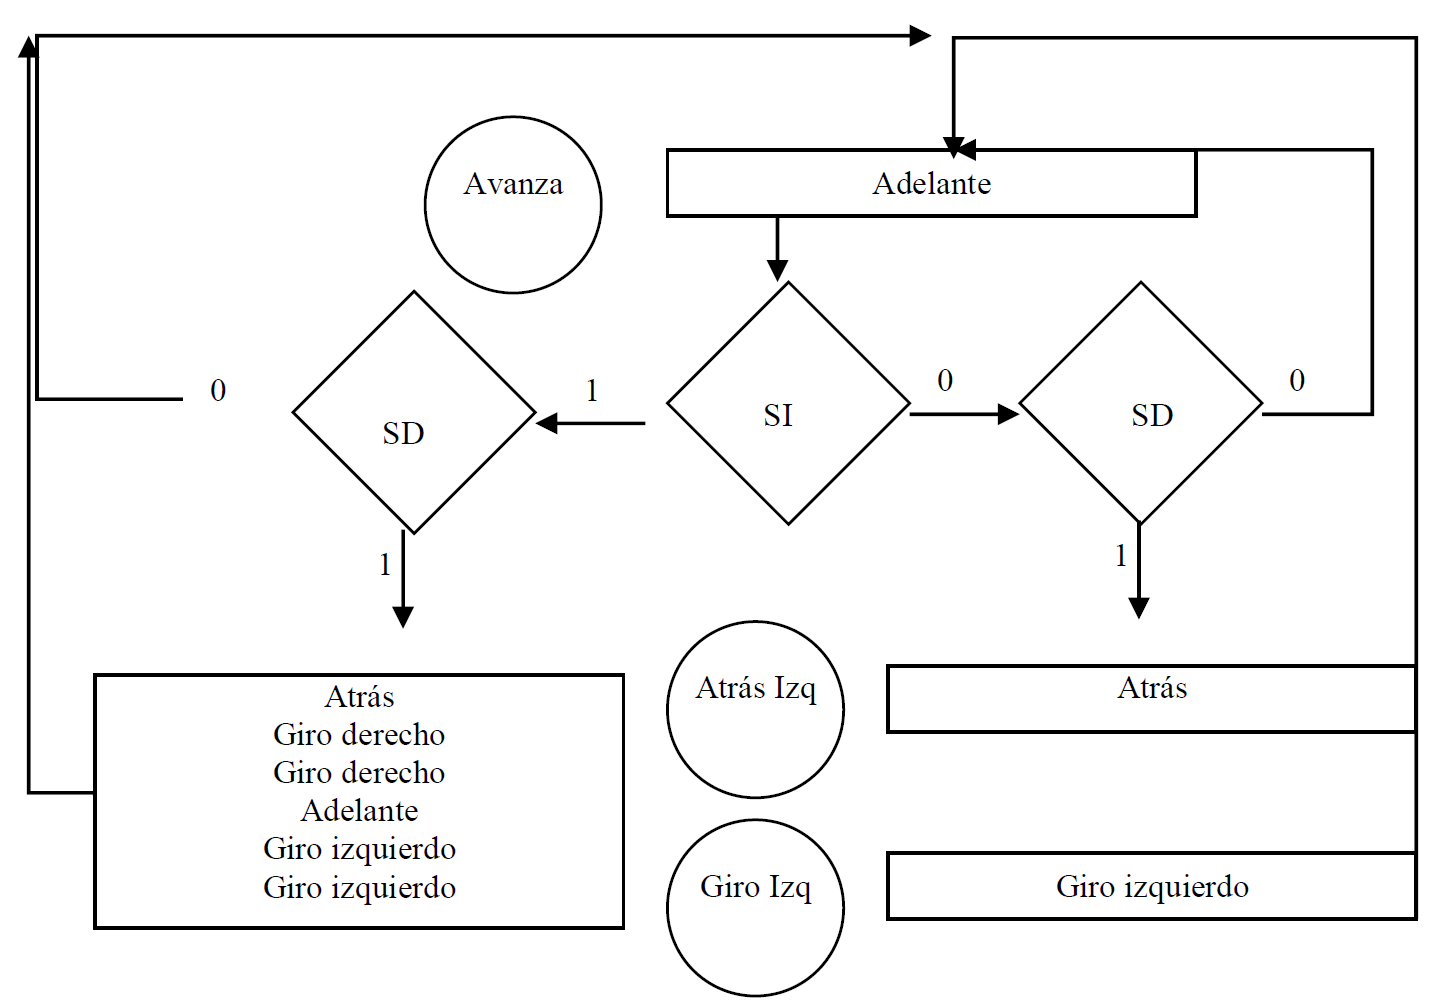
\includegraphics[width=0.5\textwidth]{images/img56.png}
	\label{figura56}
	
\end{figure}
\break

Si se quisiera programar esto con una subrutina, hace todo.  En la teoría de comportamientos necesito una respuesta inmediata y necesito que cuando vuelva a entrar se guarde el estado.

\section{AFSM (Augmented Finite State Machine)}

La máquina de estados aplicada a robots representa el comportamiento.
Una máquina tradicional de estados tiene entradas y salidas.
Rodney Brooks (MIT) inventó la máquina de estados finitos aumentada.

Básicamente el concepto es que alguna de las entradas es inhibida por otra máquina de estados (su salida se convierte la entrada) y en las salidas están los supresores, que bloquean la salida de la máquina y colocan un valor. Por último hay una entrada de “reset” que hace que se coloque en un estado en específico.

Con AFSM podemos tener diferentes capas y hacer una respuesta \textbf{jerárquica}.

\begin{figure}[h!]
	\centering
	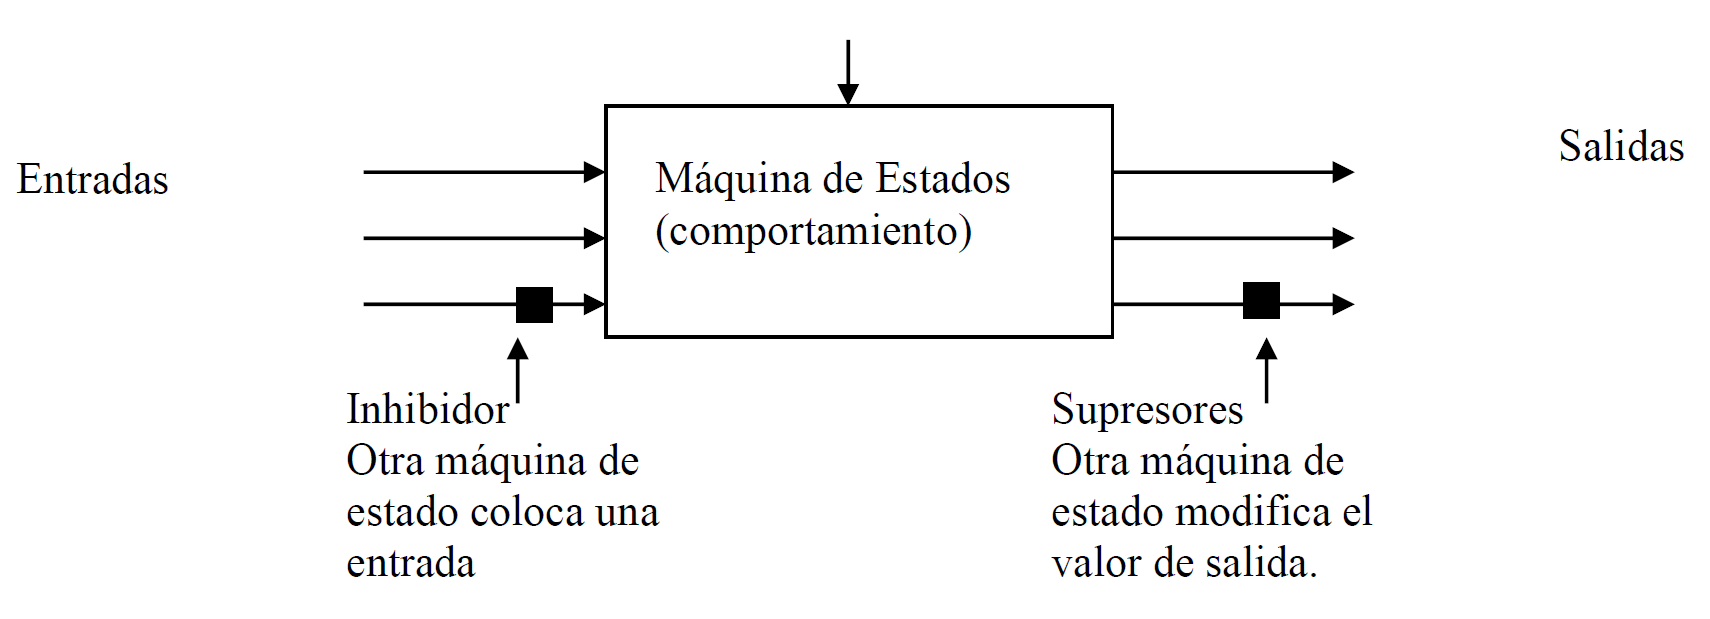
\includegraphics[width=0.5\textwidth]{images/img57.png}
	\label{figura57}
	
\end{figure}
\break

\section{Campos Potenciales}

Se modela el robot como una canica. Los obstáculos ahora son montañas que ejercen fuerzas de repulsión. El destino es un hoyo.
El robot se mueve a través de un campo potencial por la pendiente más pronunciada hasta que lo lleva al destino.

\begin{figure}[h!]
	\centering
	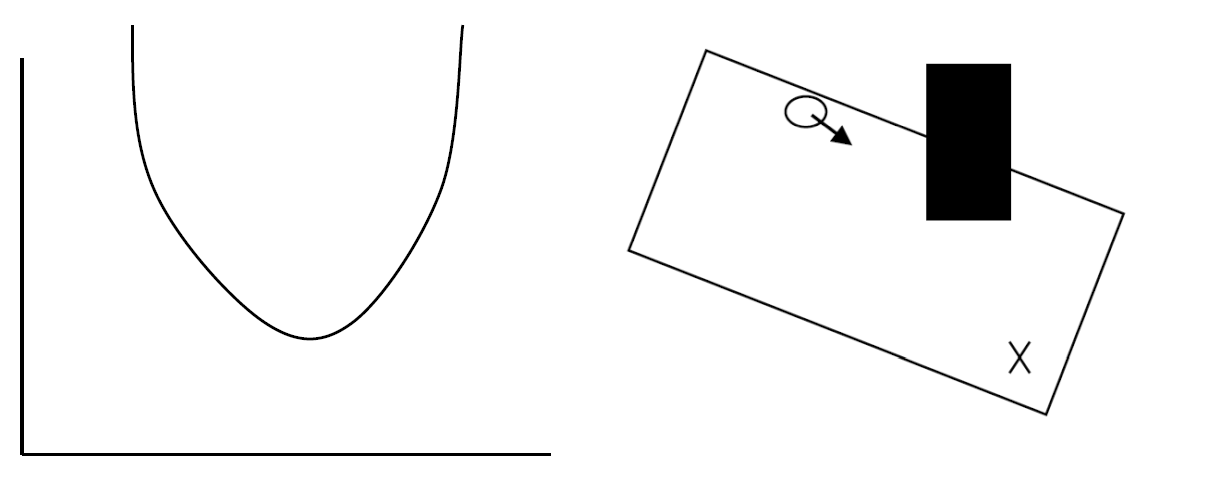
\includegraphics[width=0.5\textwidth]{images/img58.png}
	\label{figura58}
\end{figure}

$$
y=y_0 + (x-x_0)^2
$$


El mínimo se encuentra diferenciando.
$$
\dfrac{\partial y}{\partial x} = 2(x-x_0)
$$
$$
x^* = x_0
$$

Supongamos que no se conoce la ecuación; entonces se utiliza un método iterativo.
Empiezo con un punto $x_{n-1}$ cualquiera y dependiendo del valor de la pendiente me muevo hacia la izquierda o la derecha.

Es una relación de recurrencia:

\begin{center}
	$ x_n= \int(x_{n-1}) = x_{n-1} - \partial \dfrac{\partial y}{\partial x} $ \,  donde $\partial$ es una constante.	
\end{center}

\textbf{Por ejemplo:} \\
Si consideramos $\delta = \dfrac{1}{2}$ se tiene $x_n = x_{n-1} \, \dfrac{-1}{2}(2(x_{n_1}-x_0)) = x_0$.


Esto da pie a considerar la situación general.

\textbf {Se utiliza Steepest Descent.} 

\textit{Posición del robot en n:} $q_n = \left[x_n,y_n\right]^T$
$$
q_n=q_{n-1}-\delta f (q_{n-1}) $$

donde $f(z)= \dfrac{F(z)}{\|F(z)\|} = U(z)$ y $U(z)$  es el campo potencial del medio ambiente en donde navega el robot $U(z)= U_{atr}(z) + U_{rep}(z)$ (dos componentes, uno atractor y un repulsor).

Al final se tienen fuerzas de atracción más fuerzas de repulsión.

Se define:

$U_{atr} = \dfrac{1}{2} \, \varepsilon_1 \,  \|q-q_{dest}\|^2 $(campo de tipo parabólico) donde $q_{dest}$  es la posición del destino. 
Se ve claro que es parabólico:

$$
U_{atr}=\frac{1}{2} \, \varepsilon_1(x-x_{dest})^2 + (y-y_{dest})^2
$$
La fuerza de atracción en q es:

$$
\nabla U_{atr}= \varepsilon_1 \begin{bmatrix}(x-x_{dest}) \\ (y-y_{dest}) \end{bmatrix} = \varepsilon_1[q-q_{dest}] = F_{atr}(q)
$$



La fuerza de atracción se va a convertir en aceleración. Para fuerzas muy grandes se transforma en aceleraciones muy grandes. 
Esto no se quiere, por lo que se tiene un umbral. Esta fórmula solamente aplica para $\|q-q_{dest}\| < d_1$.

¿Qué pasa en $\|q-q_{dest}\|>d_1$?

$$
U_{atr}=E_2\|q-q_{dest}\|
$$

Esto es un campo cónico:

$$
U_{atr}=E_2\sqrt{(x-x_{dest})^2 + (y-y_{dest})^2)}
$$

$$
\nabla U_{atr} = E_2 \begin{bmatrix} \dfrac{(x-x_{dest})}{\sqrt{(x-x_{dest})^2+(y-y_{dest})^2}} \\ 
\dfrac{(y-y_{dest})}{\sqrt{(x-x_{dest})^2+(y-y_{dest})^2}}
\end{bmatrix} = \dfrac{E_2}{\rVert q-q_{dest}\lVert}
\begin{bmatrix}
x-x_{dest} \\
y-y_{dest}
\end{bmatrix} = E_2 \dfrac{q-q_{dest}}{\lVert q-q_{dest}\rVert}
$$

Campos Repulsivos

¿Cómo representar el obstáculo? Se podría considerar un solo vector en el centroide, una serie de puntos que ejercen repulsión, etc. Depende del diseñador.

$$U_{rep}(q)=\frac{1}{2}\eta \left( \dfrac{1}{\lVert q-q_{obs}\rVert} - \dfrac{1}{d_0} \right) ^2 $$

Esto aplica cuando $q-q_{obs}$. En caso contrario, se toma como 0. Esto es para que no lo tomes en cuenta si está demasiado lejos.

$$
\nabla U_{rep}(q)=-\dfrac{\eta}{\rVert q-q_{obs}\lVert ^2} \left( \dfrac{1}{\lVert q-q_{obs}\rVert} - \dfrac{1}{d_0} \right)
\left( \dfrac{q-q_{dest}}{\lVert q-q_{dest}\rVert}\right)
 =F_{rep}(q)
$$

En general,

$$
F(q)=F_{atr}(q)+\sum_{i=1}^{n}\, F_{rep}(q)
$$

$$
f(q)=\frac{F(q)}{\|F(q)\|}=\nabla U(q)
$$

$$
q_{i+1}=q_i - \delta_i f(q_i)
$$

\begin{figure}[h!]
	\centering
	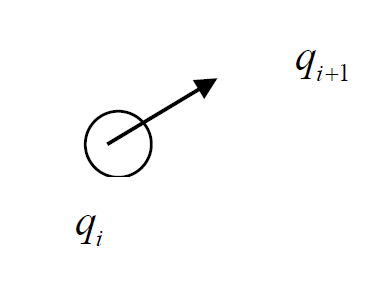
\includegraphics[width=0.3\textwidth]{images/img59.png}
	\label{figura59}
\end{figure}



\begin{ejemplo}
	Robot:(1,1) \\
	Obstáculo: hexágono centrado en (2,2) \\
	Objetivo:(5,4) \\
	$q_0=(1,1)$\\
	Se va a tomar $d_0=	5, \varepsilon_1=1, \eta=2,\delta_0=1$ y se va a utilizar la parabólica
\end{ejemplo}

Se tiene: 

%EJEMPLO
$$
\begin{array}{rcl}
F_{atr}(q_0) & = & \varepsilon_1 (q_0-q_{dest}) \\
             & = &  (-4,-3)
             
             
\end{array}
$$

$$
F(q_0) = - \dfrac{\eta}{\rVert q_0 - q_{obs} \lVert^2} \left(\dfrac{1}{\lVert q_0-q_{obs}\rVert} - \dfrac{1}{d_0} \right)
\left( \dfrac{q_0 - q_{obs}}{\lVert q_0 - q_{obs}\rVert}\right)
$$

$$
= \dfrac {-2}{\sqrt{2}} 
\left(\dfrac{1}{\sqrt{2}} - \dfrac{1}{5}\right) \left(\dfrac{1}{2\sqrt{2}} \right) (-1,-1)
$$


$$=-(0\ldotp3585,0\ldotp3585)$$

La fuerza total es: 



$$
F(q_0) =(-3\ldotp64,-2\ldotp64) \hspace{0.5cm} f(q_0)=(-0\ldotp8091,-0\ldotp 5868)
$$
Finalmente:

%\begin{eqnarray*}
%$$
%q_1 = q_0-\delta_0 (q_0) \\
% = (1,1)+(0\ldotp8091.0\ldotp5868) \\
% = (1\ldotp8091,1\ldotp5868) 
%$$
%\end{eqnarray*}

\begin{equation*}
\begin{aligned}
q_1 & = \,  q_0-\delta_0 (q_0) \\
 & = \, (1,1)+(0\ldotp8091.0\ldotp5868) \\
 & = \, (1\ldotp8091,1\ldotp5868) 
\end{aligned}
\end{equation*}

Obsérvese que no hemos considerado la \textbf{orientación inicial del robot}.



¿Cómo encontrar las constantes? Empíricamente

Nota: Si no conocemos obstáculos no podemos calcular las fuerzas de repulsión. En estos casos, se tiene que usar la información de los sensores para identificar al obstáculo y, con base en eso, calcular estas fuerzas.

\textbf{Cálculo de los vectores de repulsión usando la posición de los obstáculos fijos}

Los obstáculos conocidos se representarán por polígonos que tienen nodos ordenados en el sentido de las manecillas del reloj.

El espacio se divide en celdas y en cada celda se calcula la fuerza total de repulsión.

\begin{figure}[h!]
	\centering
	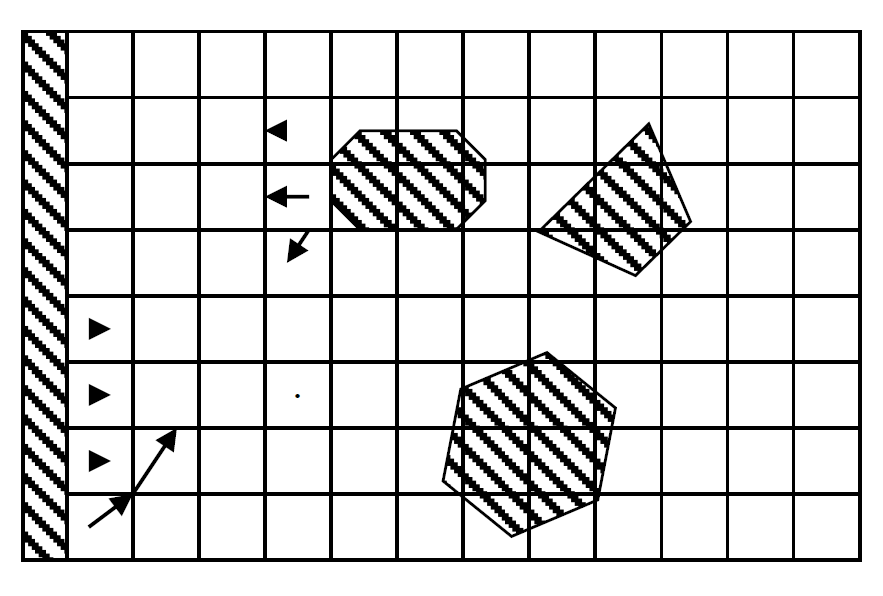
\includegraphics[width=0.5\textwidth]{images/img60.png}
	\label{figura60}
\end{figure}

Etc.

¿Cómo encontrar la fuerza de repulsión en cada celda?

\begin{figure}[h!]
	\centering
	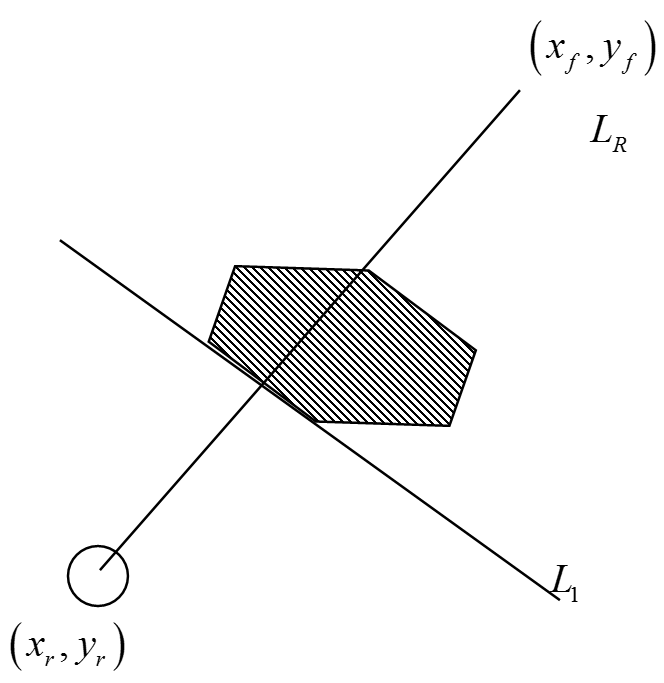
\includegraphics[width=0.5\textwidth]{images/img61.png}
	\label{figura61}
\end{figure}

El punto $x_r,y_r$ es el centro de la celda en donde se está (se asume que el robot está en el centro de la celda).

El punto $(x_f,y_f)$ es  un punto arbitrario (se quiere calcular para la mayor cantidad de direcciones posibles.
No es en línea sino que se hace offline).


\begin{flalign*}
\begin{aligned}
 L_1:\colon y=m_1x+b_1 \\
 L_R:y=m_Rx+b_R
\end{aligned}
\end{flalign*}


Nótese que 

\begin{flalign*}
\begin{aligned}
x_f=d\cos\phi+x_r \\
y_f=d\sin\phi+y_r
\end{aligned}
\end{flalign*}

Donde el ángulo es entre el eje x y la línea $L_R$.

Obs: se puede encontrar

$$
m=\dfrac{y_1-y_0}{x_1-x_0} \hspace{0.5cm} b=\frac{x_1y_0-y_1x_0}{x_1-x_0}
$$

Los puntos de intersección son

$$
x_{int}=\frac{b_r-b_1}{m_1-m_r} \hspace{0.5cm} y_{int}=m_r x_{int} + b_r
$$

Obsérvese que se tiene que cumplir que $x_{int} \in(x_0,x_1)$ y$y_{int} \in(y_0.y_1)$

\section{Cómo calcular el campo potencial para el caso de objetos desconocidos}

Lo anterior se hace offline y se alimenta al robot. Si hay objetos desconocidos:

\begin{figure}[h!]
	\centering
	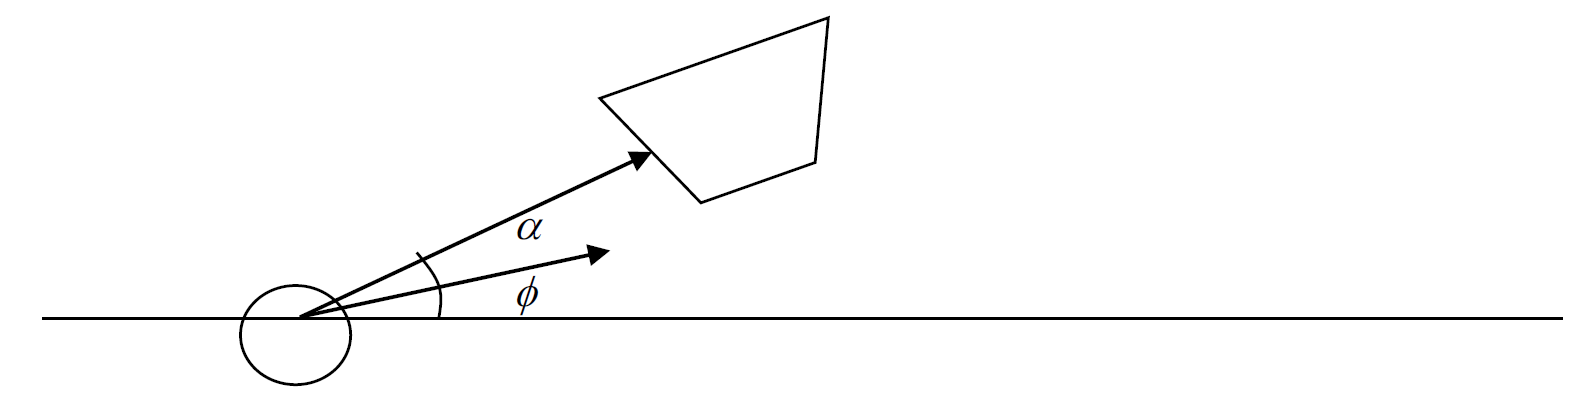
\includegraphics[width=0.5\textwidth]{images/img62.png}
	\label{figura62}
\end{figure}

\begin{scaja}
Tarea 1 \\
Usar Roc2. Poner obstáculos pickable en el medio. Programar un robot para encontrar esos obstáculos y que
los lleve a un lugar. Usar nada más la parte rectangular del mundo. El robot se mueve aleatoriamente. Tener
una pila que se vaya bajando.
\end{scaja}



¿Qué se quiere? \\
De $(x_{i-1},y_{i-1},\phi_{i-|})$ (donde está el robot) necesito llegar a $(x_i,y_i,\phi_i)$.

Obsérvese que: \\
 $x_i=x_{i-1}+x_i \cos(\phi_i)
 y_i=y_{i-1}+x_i \sin(\phi_i)
 $
 
donde:

$
\phi=\phi_{i-1}+\phi_i \\
\phi=\arctan\ (\frac{y_i -y_{i-1}}{x_i -x_{i-1}})
$


Esto se conoce como \textbf{computación directa}.

Otra opción es:

$
x'_i= \dfrac{(x_i - x_{i-1}) + (y_i - y_{i-1})}{\cos(\phi_i) + \sin(\phi_i)}
$

$
\phi_i = \phi_i - \phi_{i-1}
$
y obviamente también se tiene que $x_i = \sqrt{(x_i - x_{i-1})^2 + (y_i - y_{i-1})^2 }$



Esto se llama \textbf{computación inversa} y es la que nos interesa.



\textbf{Ejemplo}



\begin{figure}[h!]
	\centering
	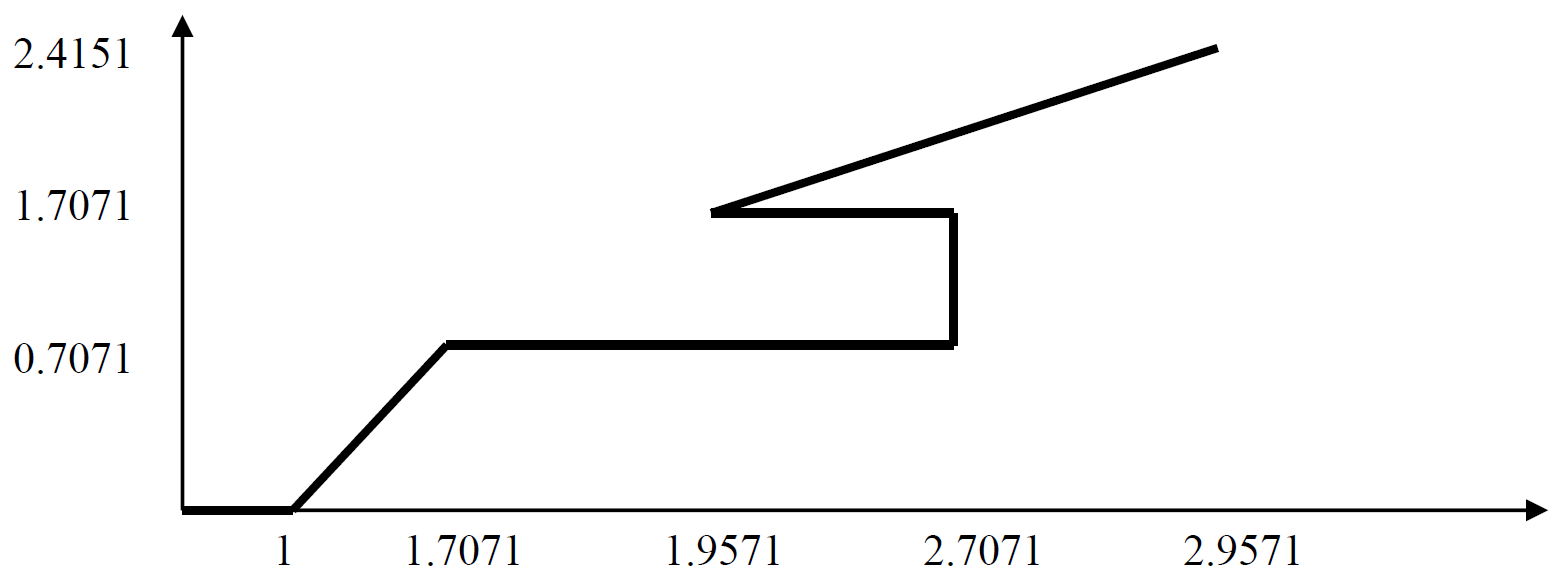
\includegraphics[width=0.5\textwidth]{images/img63.png}
	\label{figura63}
\end{figure}


\underline{Sup:} Los puntos los encontré con campos potenciales (recordar que el campo potencial da el vector de
movimiento:

$q_1=(x_i,y_i) = q_{i-1} - \delta f (q_{i-1})$
\\ \\
$ i=1 $ \\
$ x_0 = 0, \hspace{0.5cm} y_0=0, \hspace{0.5cm} \phi_0=0 $ \\
$x_i =1 \hspace{0.5cm} y_i=0 $

Por lo tanto: $\phi_1 =  arctan \, \left( \dfrac{y_1-y_0}{x_1-x_0} \right) = 0 \hspace{0.3cm} y \hspace{0.3cm} x_1 = \sqrt{(x_1-x_0)^2 + (y_1-y_0)^2} = 1.$ Y finalmente: \hspace{0.3cm} $\phi_i=\phi_i-\phi_{i-1} = 0$

Ad nauseam. \\
Los valores son:

\begin{figure}[h!]
	\centering
	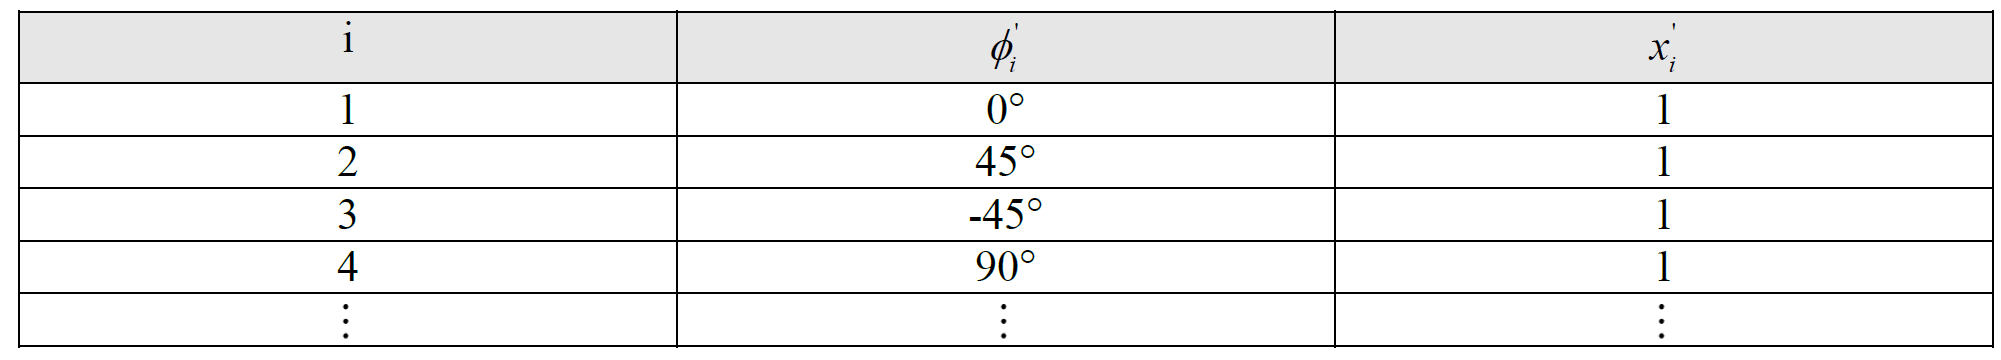
\includegraphics[width=0.5\textwidth]{images/img64.png}
	\label{figura64}
\end{figure}



\subsection{Trayectorias}

El robot casi siempre avanza en línea recta. \\
¿A qué velocidad debe ir el robot?

El robot está en $(x_{i-1},y_{i-1},\phi_{i-1}) $y quiero llegar a $(x_i,y_i)$ .¿Cómo voy a recorrer la distancia $x_i$?
Tengo $t_0$ y el tiempo $t_f$ (final).


\begin{figure}[h!]
	\centering
	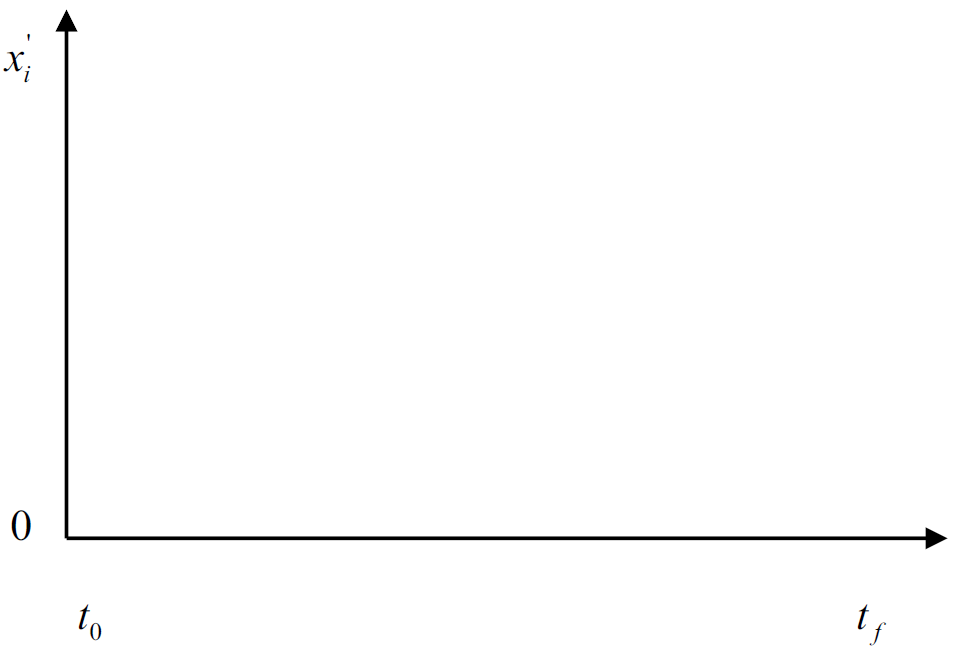
\includegraphics[width=0.5\textwidth]{images/img65.png}
	\label{figura65}
\end{figure}


Se quiere una función $f(t)$ que sea suave. Se asume que el robot está parado en ambos extremos.

$f(0)=0, \, f(t_f)= x_i' \hspace{0.3cm}$ [posiciones inicial y final]

$f'(0)=0, \, f'(t_f)= x_i $ \hspace{0.3cm}[velocidades inicial y final]


Asumiendo una relación cúbica:

$f(t)=a_0 +a_it + a_2 t^2 + a_3 t^3 \, f'(t_f)= x_i$

$f'(t)=a_1 + 2a_2t + 3a_3 t^2$

$f''(t)=2a_2 + 6a_3t$

Se encuentran:

$a_0, a_1=0, a_2=\dfrac{3x_i}{t_f^2},a_2=\dfrac{-2x_i}{t_f^3}$. La ecuación es entonces:
$$
f(t)=\dfrac{3x_i}{t_{f}^2}t^2 - \dfrac{2x'_{i}}{t_{f}^2} t^3
$$

$$
f'(t)=\dfrac{6x_i}{t_{f}^2}t -  \dfrac{6x'_{i}}{t_{f}^2} t^2
$$

$$
f''(t)=\dfrac{6x_i}{t_{f}^2}- \dfrac{12x'_{i}}{t_{f}^2} t
$$

\begin{ejemplo}
	
	
	Suponer $ t_f = 3 \,  x_1=1$ \\
	Entonces
	
	$$f(t)=\dfrac{1}{3}t^2 - \dfrac{2}{27}t^3
	$$
	
	$$f'(t)=\dfrac{2}{3}t - \dfrac{6}{27}t^2$$
	
	$$f''(t)=\dfrac{2}{3} - \dfrac{12}{27}t$$
	
\end{ejemplo}


\begin{figure}[h!]
	\centering
	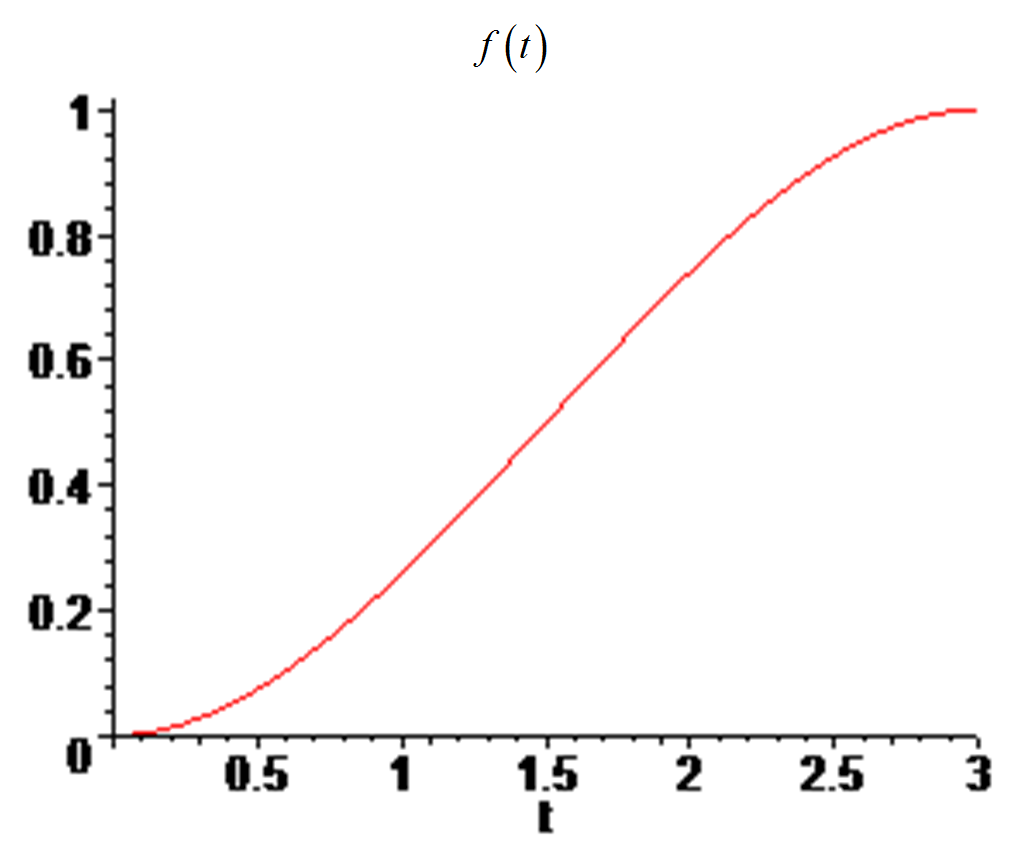
\includegraphics[width=0.5\textwidth]{images/img66.png}
	\label{figura66}
\end{figure}


$$
f'(t)$$
\begin{figure}[h!]
	\centering
	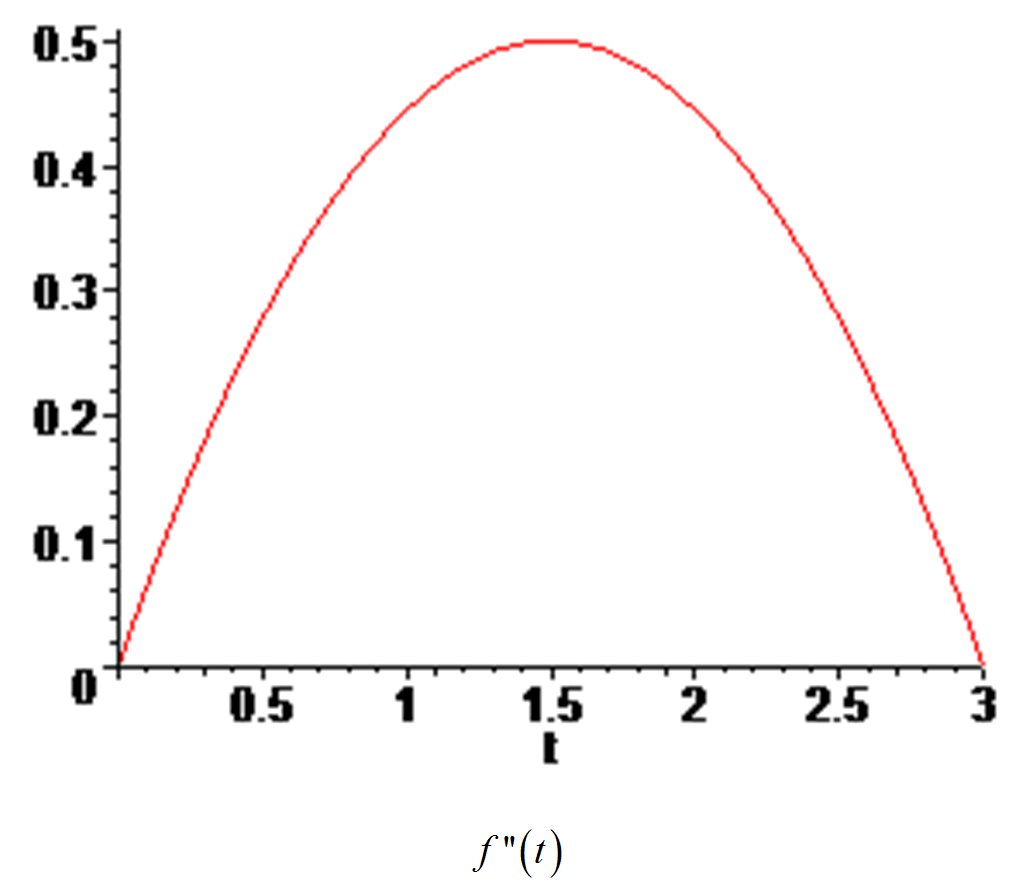
\includegraphics[width=0.5\textwidth]{images/img67.png}
	\label{figura67}
\end{figure}


\begin{figure}[h!]
	\centering
	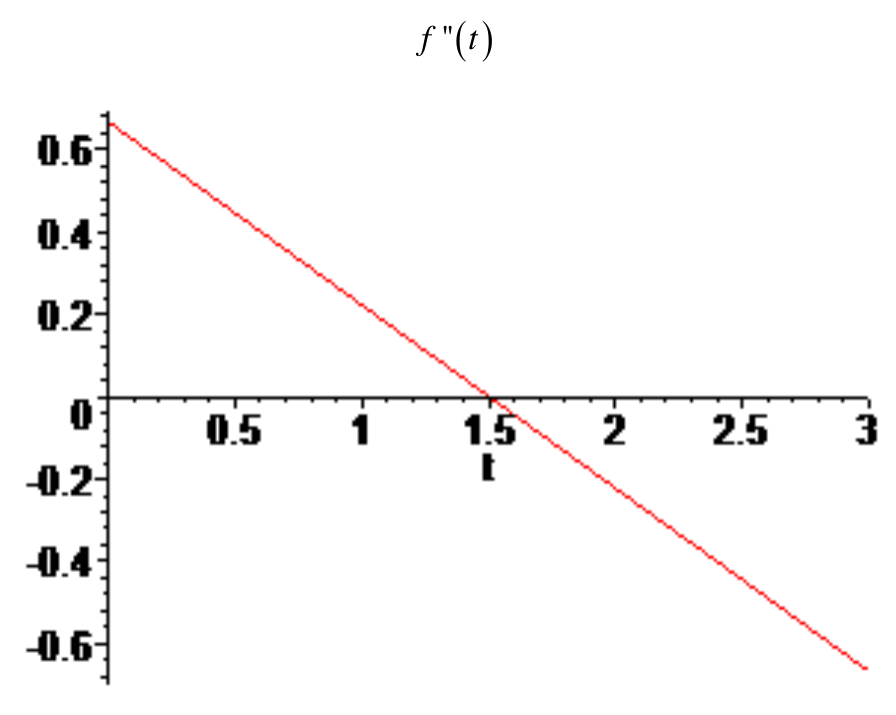
\includegraphics[width=0.5\textwidth]{images/img68.png}
	\label{figura68}
\end{figure}


En Roc2 para mover es:

mv $x'_i \hspace{0.3cm} \phi_i\hspace{0.3cm}t_f$

donde la primera está dada en decímetros y el ángulo en radianes y el tiempo en segundos.

En Roc2 las funciones cinemáticas se encuentran en el archivo Roc2UserMv.

\underline{\textit{Cómo relajar el supuesto de la velocidad final 0}}

Suavizar la trayectoria.

\begin{scaja} 
	
	Una forma: Le ajustas una parábola a la esquinita
	$y=y_0 + (x-x_0)^2$ con $x_b \leq x \leq x_f $ puntos pre-escogidos.
	
	\vspace{5mm}
	
	Otra forma: linearizar (segmentitos de recta).
	
\end{scaja}

\textbf{Rotar y trasladar}

polygon type-object $(x0,  y0, x1, \, y1, \, x2, \, y2, \, ... yn yn)$
position \textit{room} type-object name $xc yc theta ) \leftarrow$ esta función traslada a xc, yc y rota theta
Type-object define un objeto genérico, podemos definir varios objetos (de ese tipo).

\vspace{5mm}
Dados $(x_p,y_p)$


$ x= x_p \cos\alpha - y_p \sin\alpha +x_c $

$y = y_p \cos\alpha + x_p \sin\alpha +y_c$

Donde $x_c$, $y_c$ es el punto fijo sobre el que se está girando.

\begin{ejemplo}
	Polygon mesa $1 \, 0 \, 0\, 0\, 2\, 2\, 2\, 2\, 0$ \\	
	Position salon mesa1 mesa\_principal 44 $\frac{\pi}{4}$
\end{ejemplo}

Entonces:

\begin{figure}[h!]
	\centering
	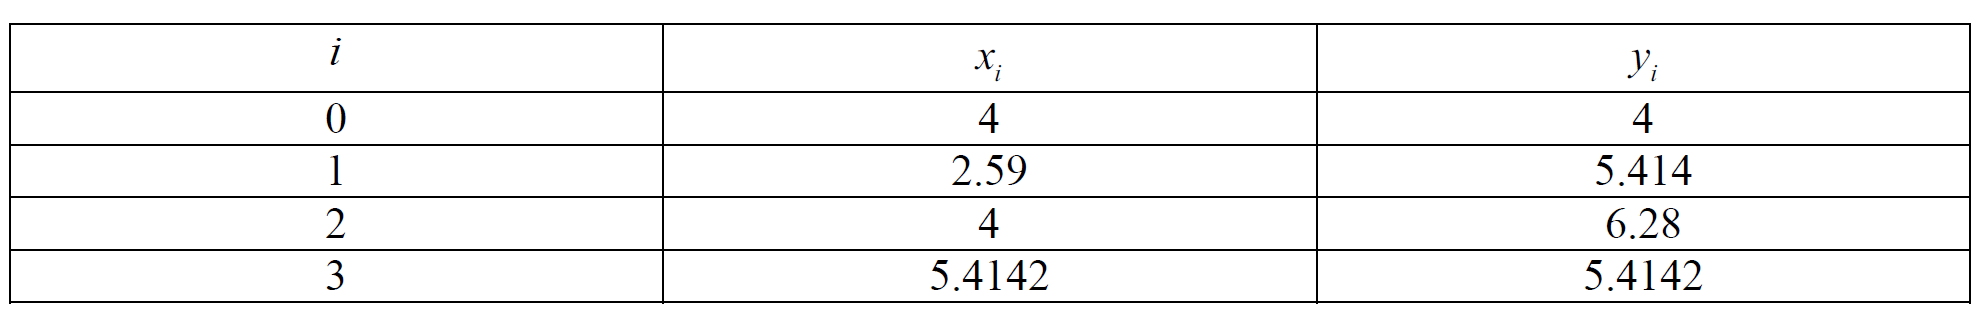
\includegraphics[width=0.5\textwidth]{images/img69.png}
	\label{figura69}
\end{figure}

\textbf{Ancho del robot}
Se necesita considerar el ancho del robot. Por lo menos, ensanchar los obstáculos conocidos en el radio del
robot.
¿Cómo hacer con los desconocidos? De la lectura del sonar, restarle el radio del robot.

\section{Escalamiento de polígonos}

Suponer (0, 2), (1,3), (2, 2), (1,1) un polígono.


\begin{enumerate}[1.]
	\item Encontrar el centroide
	\item Moverlo al origen
	\item Multiplicar
	\item Volverlo a mover al centroide.
\end{enumerate}


Con $\lambda =2$


$P_esc = \lambda (P - C) + C$

$P = \{(-1,2),(1,4),(3,2),(1,0)\}$

\begin{scaja}
	\textbf{Siguiente tarea}
	
	El mundo tiene mesas y otros dos objetos tipo, puestas y rotadas.
	
	Objetos fijos: sillones, mesas, cajas, etc. (al menos 3)
	\\
	
	Descomponer el mundo en celdas.
	\\
	
	Calcular los vectores de repulsión en cada celda.
	Si el centroide de la celda queda dentro del obstáculo, está ocupada
	Hacer una “estrella” hacia todas las direcciones y calcular si la intersección con algo es menor o igual a d0.
	\\
	La repulsión total es la suma.
	\\	
	
	Tres archivos: 1) objetos tipo 2) posiciones objetos réplica 3) archivo final .WRL con la descripción del
	mundo.
\end{scaja}

\textbf{Verificación de si un punto está dentro o fuera de un polígono}

\begin{figure}[h!]
	\centering
	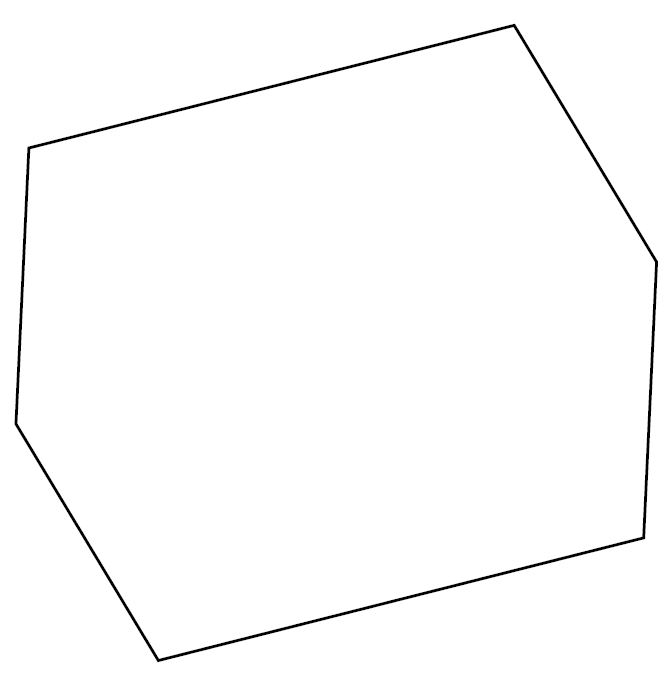
\includegraphics[width=0.3\textwidth]{images/img70.png}
	\label{figura70}
\end{figure}
	%\break

Ecuación paramétrica de la recta
$
x = x_0 + (x_1 - x_0)t \\
y = y_0 + (y_1 - y_0)t \\
t \in (0,1)
$

Los puntos de la ecuación general

$
(y_0 - y_1)x + (x_1 - x_0)y + (x_oy_1 - x_1y_0) = 0
$

Puntos que cumplen esta ecuación, están en la línea.
\\ Puntos que evalúan >0, caen a la izquierda. \\ Puntos que evalúan <0, caen a la derecha.

\textbf{Problema de los campos potenciales}
\\ Por ejemplo un mínimo local


\begin{figure}[h!]
	\centering
	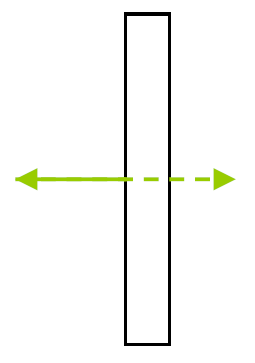
\includegraphics[width=0.3\textwidth]{images/img71.png}
	\label{figura71}
\end{figure}
%\break


El vector resultante es 0 y el robot se queda inmóvil o en un ciclo.

\section{Comportamientos con Redes Neuronales}

Redes neuronales: 1943 $\rightarrow$  McCullock


Una red neuronal es un modelo matemático de cómo funciona una neurona.

Una neurona está conectada a otras neuronas.

\begin{figure}[h!]
	\centering
	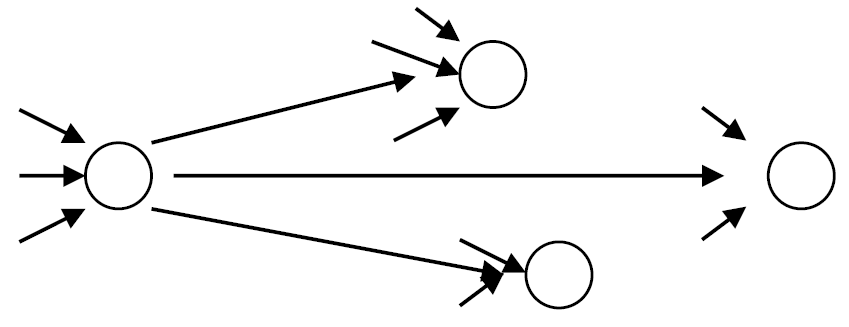
\includegraphics[width=0.5\textwidth]{images/img72.png}
	\label{figura72}
\end{figure}

La entrada a la red neuronal es una imagen (por ejemplo, la cámara del robot). Se puede entregar la
información en bruto o procesada.

Las conexiones se van uniendo por medio de aprendizaje.

Se entrena a la red para que siga los comportamientos, por ejemplo un coche autónomo. Para entrenarlo, se
puede poner a un conductor y hacer que la red aprenda los comportamientos de acuerdo a las imágenes.
La respuesta de la red es: para una cierta imagen, se giró a la izquierda violentamente; para otra imagen, se
giró ligeramente; etcétera.

También se puede hacer con información de sonares, etc.

Puedo hacer máquinas de estado con redes neuronales.

\begin{figure}[h!]
	\centering
	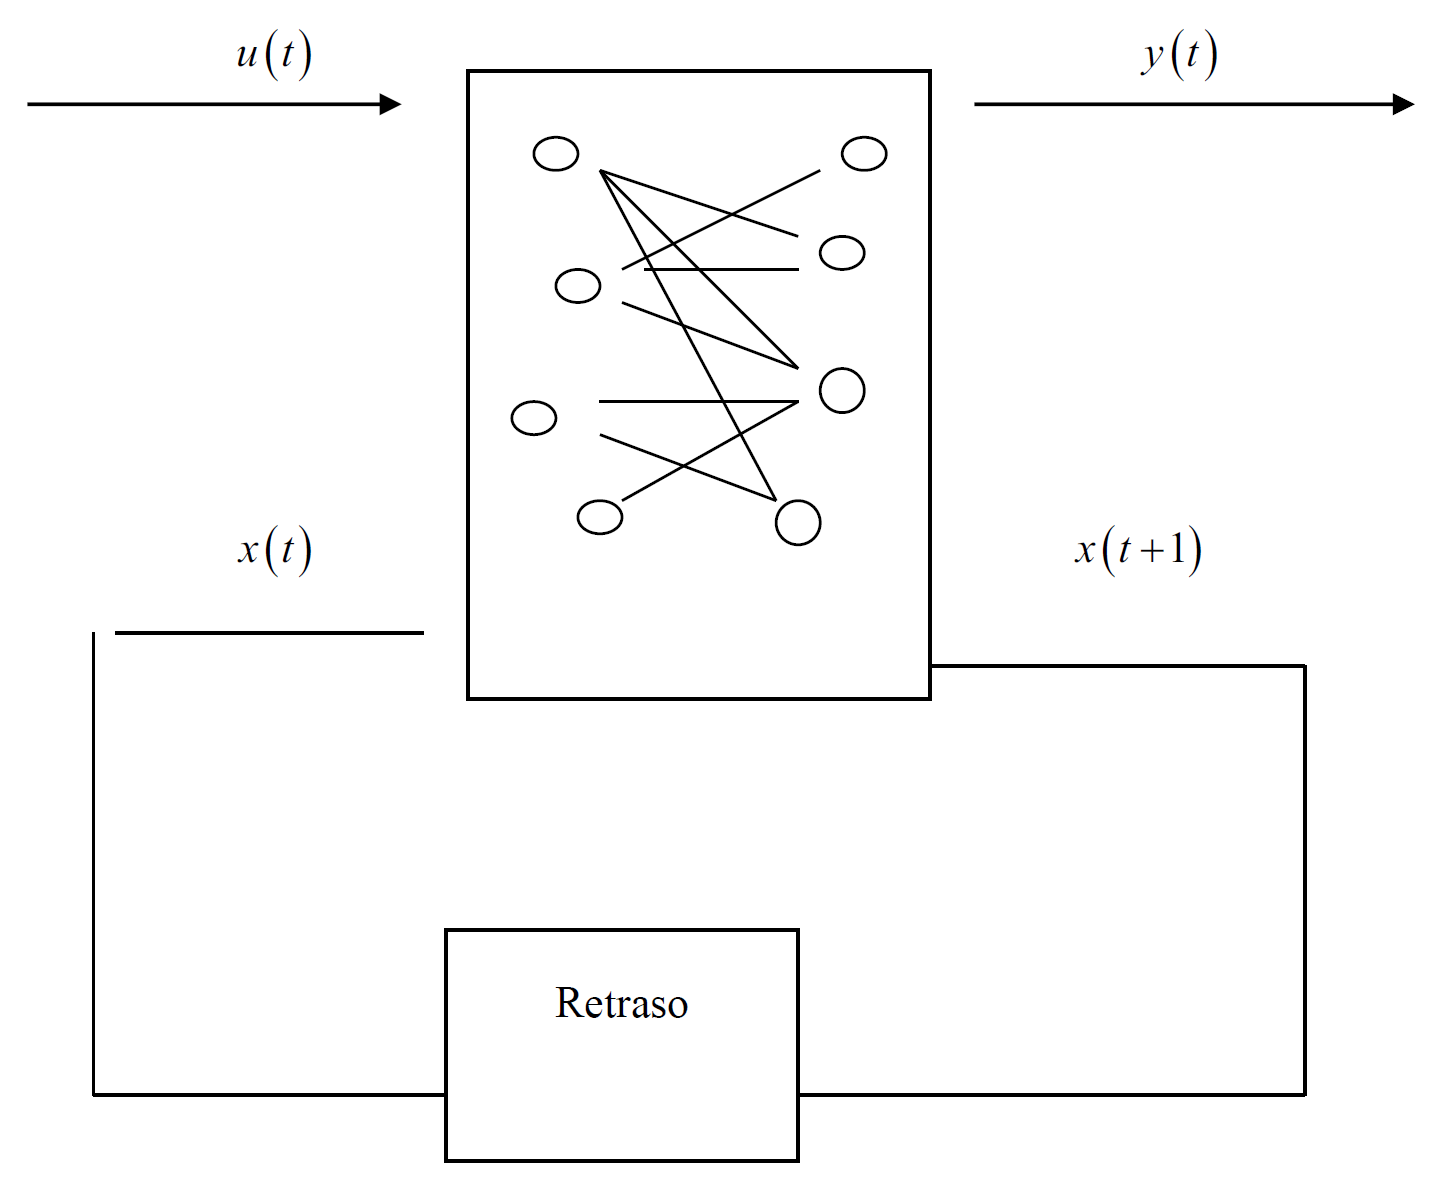
\includegraphics[width=0.5\textwidth]{images/img73.png}
	\label{figura73}
\end{figure}

\textbf{Modelo}

Por cada neurona se tiene

$u = \displaystyle \sum_{i=1}^{n} w_i\, y_i + \theta $

Entradas: $ y_j \rightarrow $  vienen de otras neuronas
Pesos: $w_j$
Umbral de activación: $ \theta $

La salida de la neurona es la \textit{función de activación}

$$
a=f(u)
$$

Generalmente $ f(u) = \dfrac{1}{1 + e^\frac{-u}{T}}$ (un sigmoide)

$T$ es una constante de temperatura. 


Resulta que f es la solución de la ecuación diferencial 

$$
\dfrac{dy}{du} = \dfrac{y(1-y)}{T}
$$


\section{Topología de Redes Neuronales}

¿Qué pasa con la topología de redes neuronales (muchas neuronas)?

\begin{figure}[h!]
	\centering
	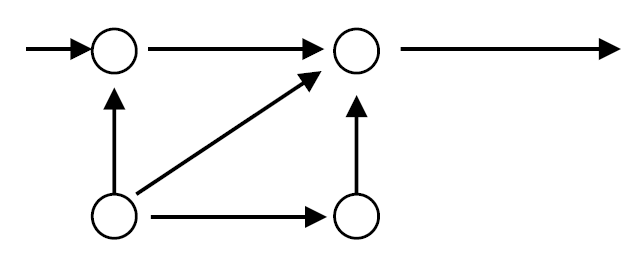
\includegraphics[width=0.5\textwidth]{images/img74.png}
	\label{figura74}
\end{figure}
\break

Topología acíclica (no hay retroalimentación de la salida hacia otra interna) $\rightarrow$ el dígrafo es acíclico.

\begin{figure}[h!]
	\centering
	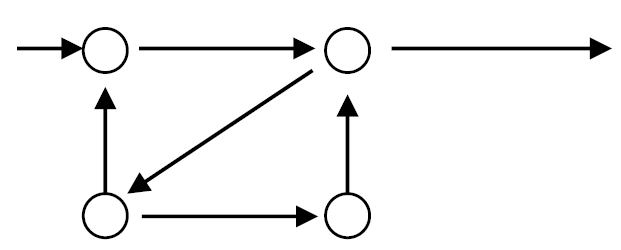
\includegraphics[width=0.5\textwidth]{images/img75.png}
	\label{figura75}
\end{figure}


Topología cíclica (con retroalimentación) $\rightarrow$ el dígrafo es cíclico
Estos fueron los primeros modelos de redes neuronales.

\section{Modelo del Perceptrón}

$
u(x) = \sum_{i=1}^{n} w_i x_i + w_0 
$
y

$
y(x) = \begin{cases}
1, \hspace{0.3cm} u(x) \geq 0    \\
0,\hspace{0.3cm}   u(x) < 0  
\end{cases}
$

Este modelo es utilizado para \textit{detección y clasificación}.

Si las características de la entrada $x$ es cercano a $w$ tal que su producto interno $x^Tw$ es mayor que un
umbral $-w_0$, entonces la salida es 1, indicando la detección de un objetivo.


\begin{ejemplo}
	Dos neuronas, una que representa una mesa y otra una silla.
	Las dos tienen las mismas entradas, que son características invariantes a distancia y orientación. La salida
	debe de ser 1 para la de la silla y 0 para la de la mesa.
\end{ejemplo}

\begin{nota} Entrenar a una red neuronal es encontrar los pesos. \end{nota}


Minsky y Shannon

Shannon propone la matemática booleana y notación binaria en las computadoras.
Wiener inventó el término \textit{cibernética} (el estudio de los sistemas – eléctricos, mecánicos, sociales, etc. – y su control).


LEER ASIMOV Y PHILIP DICK

\section{Perceptrón multicapas}

Capa de entradas
Capa intermedia
Capa de salida

\begin{figure}[h!]
	\centering
	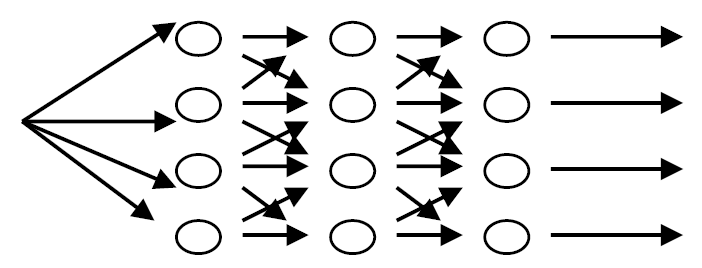
\includegraphics[width=0.5\textwidth]{images/img76.png}
	\label{figura76}
\end{figure}

La capa de entrada tiene M neuronas.
La capa intermedia se conoce como \textit{capa oculta} y tiene H neuronas.
La capa de salida tiene N neuronas.

El objetivo es encontrar los pesos que minimicen el error cuadrático medio.


Cada salida de las neuronas de salidas es un objetivo de clasificación.

\begin{ejemplo}
	
¿Cómo encontrar los pesos?

Tres entradas, una neurona de entrada.

$u=Wx$ donde $x = [1 \hspace{0.3cm} x_1 \hspace{0.3cm}  x_2]^T \hspace{0.3cm} y \hspace{0.3cm} W= [W_0 \hspace{0.3cm} w_1 \hspace{0.3cm} W_2]$
\\

Encontrar unos pesos que dado un objetivo $d_k$ e vaya actualizando con la característica que $\varepsilon \rightarrow 0$. Se
tendrán K muestras de entrenamiento $(x_k,d_k)$; salidas $z_k$ y un error total $E= \sum_{i=1}^{K}  \varepsilon_k^2$, donde $\varepsilon= d_k - z_k$.
\\

$d_k \in (0.1)$ generalmente. 

\end{ejemplo}


\begin{figure}[h!]
	\centering
	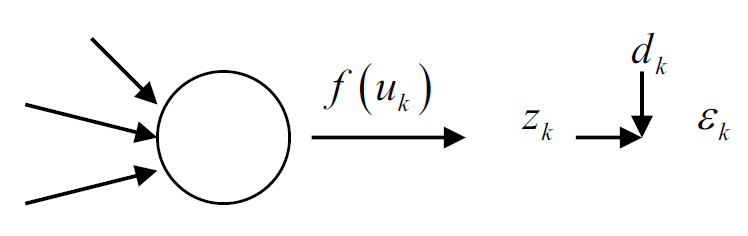
\includegraphics[width=0.5\textwidth]{images/img77.png}
	\label{figura77}
\end{figure}

Obsérvese que $z_k = f(Wx_k)$.

El objetivo final es minimizar la función $E$ respecto a $W$. 

La solución es no lineal si f es una función sigmoide, por lo que generalmente se realiza la minimización con
iteraciones:

$ W_{t+1} = W_t + \Delta W_t
$

Por método de \textit{steepest descent:}
$\Delta W_t= -\eta \dfrac{dE}{dW}
$

Solución
\\

$$
\dfrac{dE}{dW_i} = -2  \sum_{k=1}^{K}
(d_k - z_k) (\dfrac{-dZ_k}{dw_i})
$$

Obsérvese que

$$\dfrac{-dz_k}{dw_i} = \dfrac{df(u)}{dW_i} = \dfrac{df(u)}{du} \dfrac{du}{dw_i} = f'(u) \dfrac{du}{dw_i} = f'(u) x_i
$$

Por lo que

$$
\dfrac{dE}{dW_i} = 2 \sum_{k=1}^{K} (d_k - z_k) f'(u) x_i
$$

Se denota $\delta_k = [d_k - x_k] f'(u_k)$ y entonces

\begin{scaja}
	$$ w_i(t + 1) = w_i(t) + \eta \sum_{i=1}^{K} \delta_k x_i (k) $$
\end{scaja}

En particular si $f(u)$ es el sigmoide, entonces

$\delta_k=[d_k - z_k] \, z_k \,  (1-z_k)\, \alpha := \dfrac{\partial E}{\partial u}
$

\begin{scaja}
	$$ \dfrac{\partial E}{\partial u} = -2 \sum_{i=1}^{K} [d_k - z_k] \dfrac{dZ_k}{du} $$ y ademas $$\dfrac{dz_k}{du}= \dfrac{f(u)[1 - f(u)]}{T}
	$$.   \\  Por lo tanto, 
	$$
	\dfrac{\partial E}{\partial u} = -2 \sum_{i=1}^{K} [d_k - z_k] f(u) [1 - f(u)] = \dfrac{-2}{T} -2 \sum_{i=1}^{K} [d_k - z_k] \, z_k \, [1-z_k]. 
	$$
\begin{center}
	QED
\end{center}	
\end{scaja}

El proceso se debe hacer hasta que $E\textless \epsilon$


\section{Cómo extender para un perceptrón multicapas}

Se tienen:

K muestras de entrenamiento
L capas

$W_{ij}^L$ es el peso de la neurona $i$ a la neurona $j$ en la capa L y en la iteración $t$.

\textit{Propagación de error:}

\begin{figure}[h!]
	\centering
	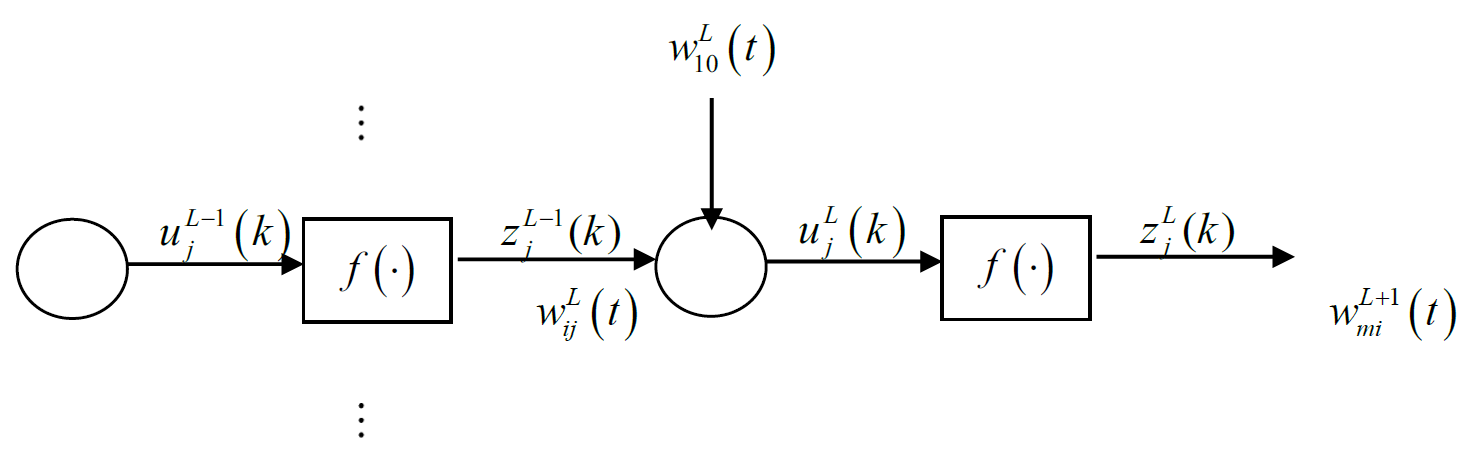
\includegraphics[width=0.5\textwidth]{images/img78.png}
	\label{figura78}
\end{figure}

El objetivo es (de nuevo) encontrar $w_ij$ de cada capa que minimicen el error cuadrático medio.

%$$ \dfrac{dE}{dw_ij^L} = -2 \sum_{i=1}^{K} \dfrac{dE}{du_i^L (k)} \dfrac{du_i^L(k)}{dw_ij^} = -2 \sum_{k=1}^{K} \delta_i^L (k) \dfrac{du_i^L(k)}{dw_ij^L}$$

Pero dado que

$
\dfrac{du_i^L (k)}{dw_{ij}^L} = \dfrac{d}{dw_{ij}^L}  \sum_{m=1}^{M} \hspace{0.2cm} w_{im}^L \hspace{0.2cm} z_{m}^{L-1} (k) 
$

%avances hasta hoy 17 

Se puede reescribir la parcial como:

$$\dfrac{dE}{dw_{ij}^L} = -2 \sum_{k=1}^{K}  \delta_{i}^L (k) z_{j}^{L-1}(k)$$
	
Se observa que el error $\delta_i^L$ en esta capa depende del error en la capa anterior, por lo que se necesita utilizar una derivación tipo Bellman para tener:

$$ \delta_{i}^L (k) = \dfrac{\partial E}{\partial u_{i}^L (k)} $$

\begin{figure}[h!]
	\centering
	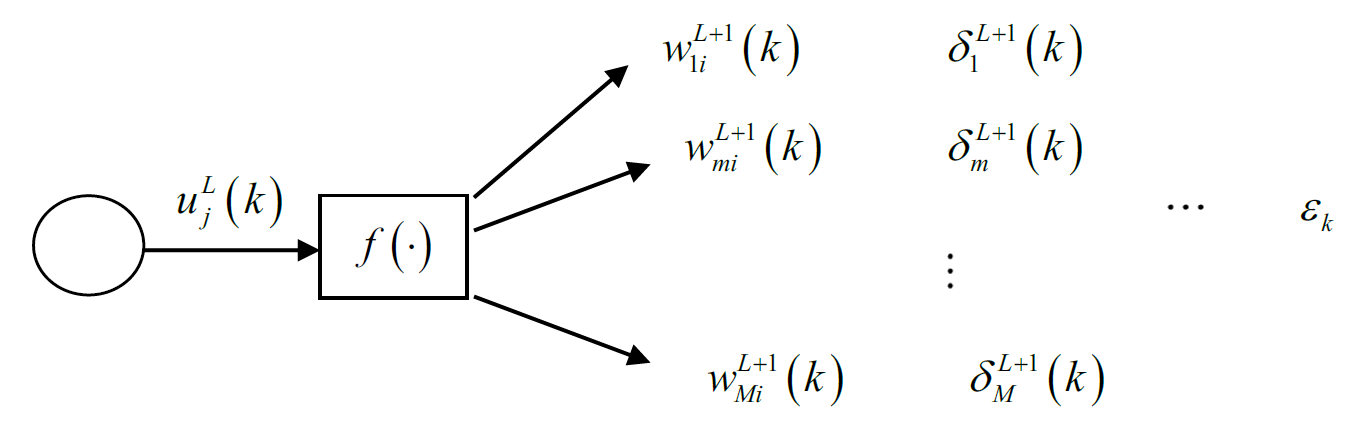
\includegraphics[width=0.5\textwidth]{images/img79.png}
	\label{figura79}
\end{figure}

Obsérvese que tiene la siguiente recursión:


\begin{equation*}
	\begin{aligned}
		 \delta_i^L (k) & = \, \dfrac{\partial E}{\partial u_{i}^L }(k) = \sum_{m=1}^{M} \dfrac{dE}{du_m^{L+1}} \dfrac{du_m^{L+1} (k)}{\partial u_i^L (k)}  \\
		& = \,\sum_{m=1}^{M} \delta_m^{L+1} (k) \left[ \dfrac{d}{\partial u_i^L (k)} \dfrac{j=1}{J} w_{mj}^L f (u_j^L (k)) \right] \\
		& = \, f'(u_i^L(k)) \sum_{m=1}^{M} \delta_m^{L+1} (k) w_{mj}^L 
	\end{aligned}
\end{equation*}

Esto se conoce como \textit{backward propagation}.

La fórmula de actualización será entonces:
\begin{figure}[h!]
	\centering
	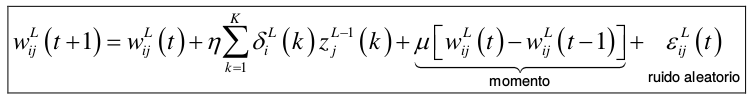
\includegraphics[width=0.9\textwidth]{images/img79_f.png}
	\label{figura79_f}
\end{figure}

La $\eta$ da la velocidad de convergencia. Sin embargo, si es muy grande, se puede dar la situación que se oscile
demasiadas veces antes de llegar al mínimo.
El error aleatorio se suma para encontrar el mínimo global.

\textbf{¿Cómo se usa esto para los robots?}

En Carnegie-Mellon University, se realizó un experimento en el cual un robot pudo manejar 90\% autónomamente en una autopista larga de Estados Unidos.

\begin{figure}[h!]
	\centering
	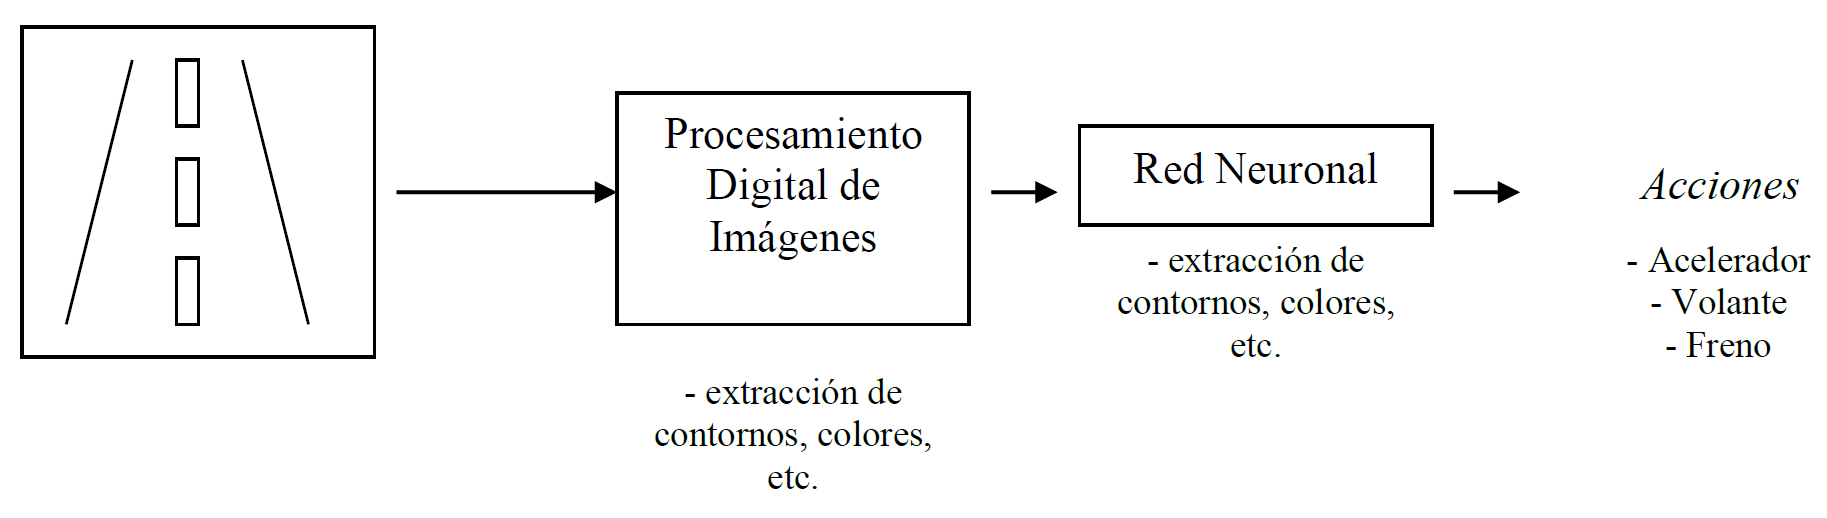
\includegraphics[width=0.9\textwidth]{images/img80.png}
	\label{figura80}
\end{figure}

El entrenamiento se haría primero manejando un humano y la red registrando qué se hizo y la foto
correspondiente.
Otra forma: máquina de estado con redes neuronales.

\textbf{Máquina de Estados con Redes Neuronales}

\begin{figure}[h!]
	\centering
	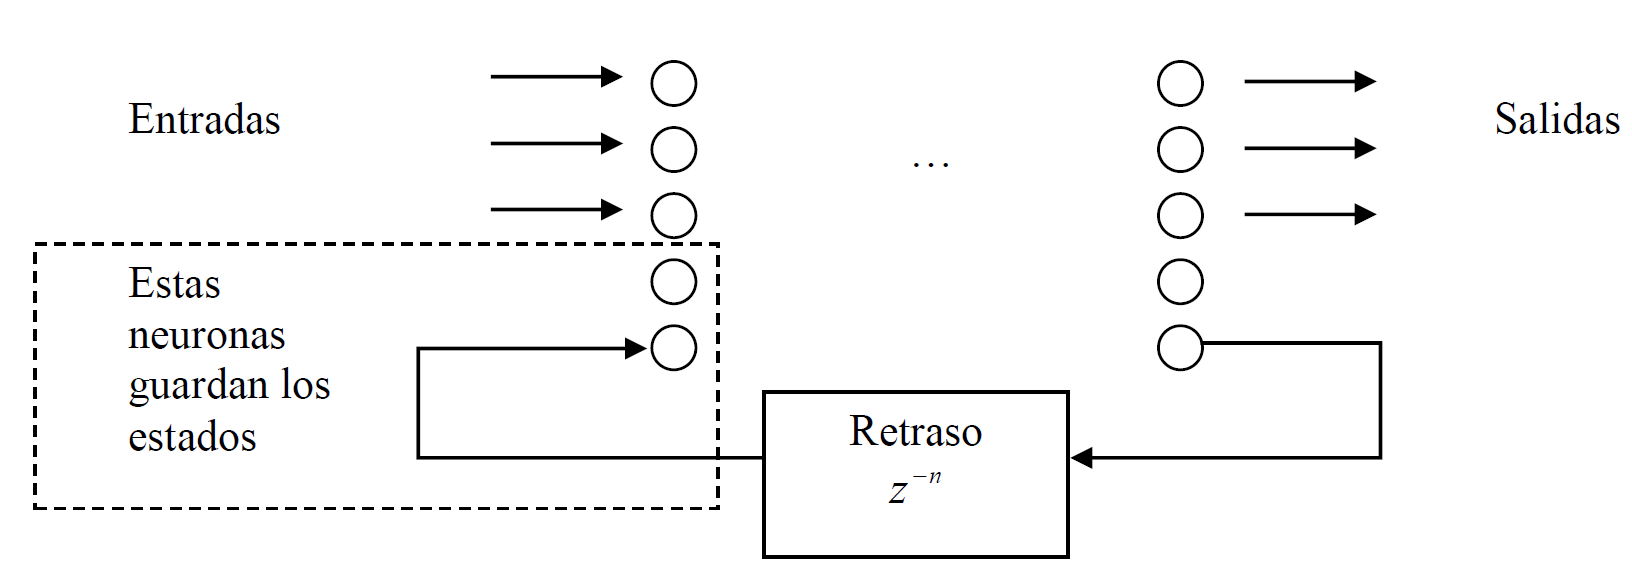
\includegraphics[width=0.9\textwidth]{images/img81.png}
	\label{figura81}
\end{figure}


\section{Aprendizaje}

El aprendizaje en un robot puede ser varias cosas:

1. Aprender “audacia”: esto depende de las constantes (afinación de constantes)
Para campos potenciales: $\mu, \delta, d_1, d_0, \eta $.

2. Aprender nuevos comportamientos

a) Crear nuevos algoritmos de máquinas de estado.

b) Modificación de las máquinas de estado \\

Hay dos cosas: una, lo que aprendemos, y otro, el conocimiento que se obtiene a través de la evolución. Por
ejemplo, un bebé sabe cómo evitar un obstáculo, no tiene que aprender. \\



\textbf{\textit{Adquisición de Comportamientos Básicos (evolución)}}

ALGORITMOS GENÉTICOS
Los algoritmos genéticos nos permitirán utilizar el concepto de evolución para:
- Afinación de constantes
- Generación de algoritmos de máquina de estado. \\


\textbf{\textit{Adquisición de Conocimiento Nuevo a partir de Comportamientos Básicos (heredados)}}

REDES NEURONALES
Aprendizaje por medio de ejemplos (tú le enseñas qué debe de hacer en determinadas circunstancias).


\textbf{¿Qué es un algoritmo genético?}

\begin{figure}[h!]
	\centering
	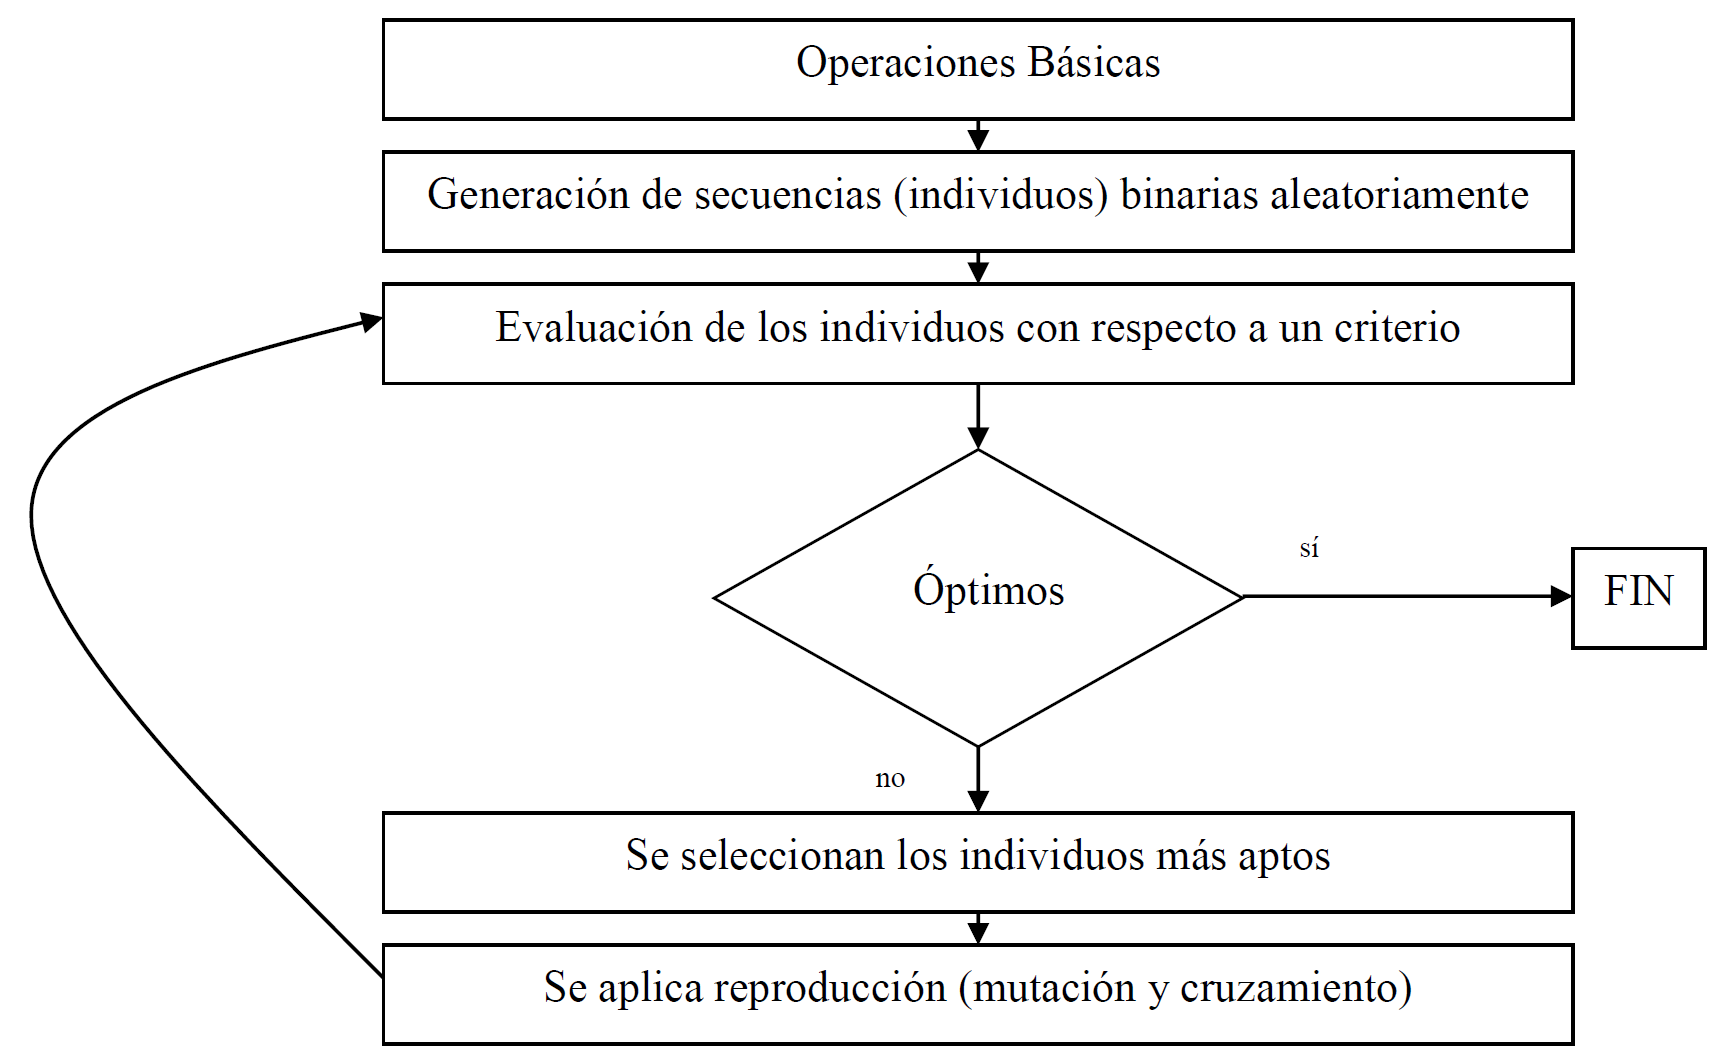
\includegraphics[width=0.9\textwidth]{images/img82.png}
	\label{figura82}
\end{figure}

Las operaciones básicas sirven para evaluar a los individuos, es decir se genera una medida para evaluar a
cada secuencia de bits.
%NOTA no se puede poner imagen :(
%\begin{ejemplo}
% 
%
%	\begin{figure}
% 
% 	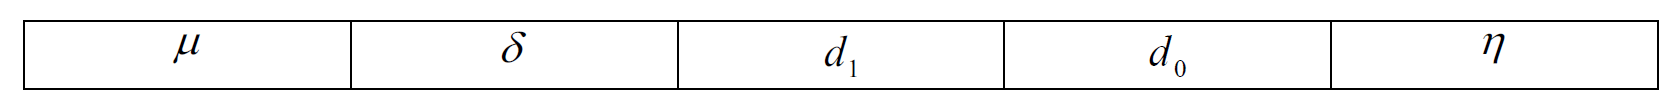
\includegraphics[width=0.9\textwidth]{images/img86.png}
% 	\label{figura86}
% 	\end{figure}
% 		
%\end{ejemplo}

\begin{figure}[h!]
\centering
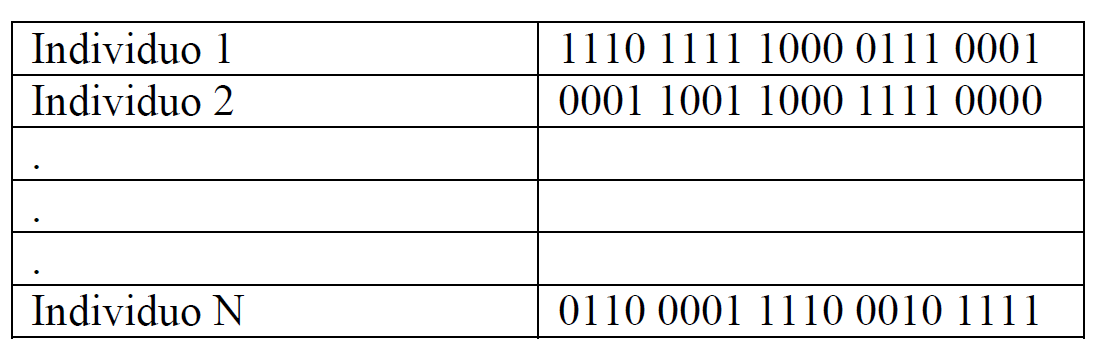
\includegraphics[width=0.9\textwidth]{images/img83.png}
\label{figura83}
\end{figure}
\break 


Ahora suponer que se cruza el individuo 1 con el 2 y tiene dos descendientes:

\begin{figure}[h!]
	\centering
	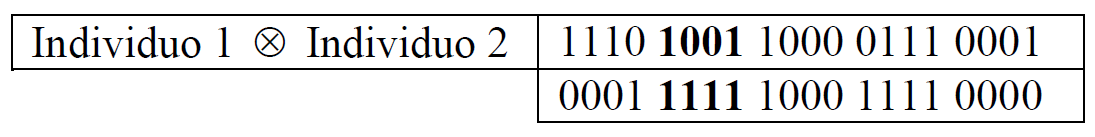
\includegraphics[width=0.9\textwidth]{images/img84.png}
	\label{figura84}
\end{figure}

Para hacerlo “realista” se tienen que tomar partecitas (bloques de bits) del mismo lugar (por ejemplo del
segundo bloque).

Mutación:

\begin{figure}[h!]
	\centering
	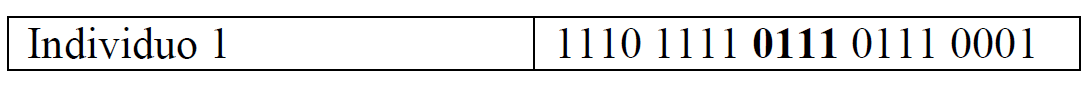
\includegraphics[width=0.9\textwidth]{images/img85.png}
	\label{figura85}
\end{figure}


\textbf{\underline{1. Afinación de Constantes en Campos Potenciales}}

Se tiene un \textbf{cromosoma} que codifica las constantes de un robot que navega usando campos potenciales.

\begin{figure}[h!]
	\centering
	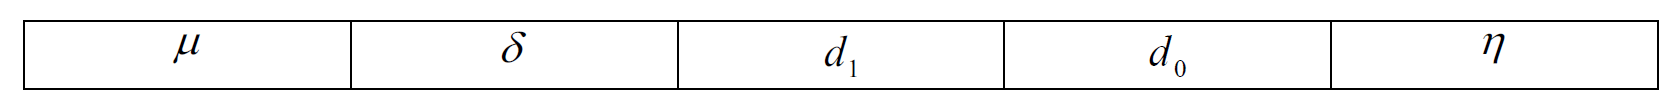
\includegraphics[width=0.9\textwidth]{images/img86.png}
	\label{figura86}
\end{figure}

Por ejemplo si $\mu = 3.5$ y se quiere tener cuatro bits para la parte entera y cuatro para la decimal:

$0011 1000$
Pues es $(0)2^3 + (0)2^2 + (1)2^0 + (1)2^{-1}$

(verificar que esto es cierto)

Si se tienen n individuos y se evalúan en un medio ambiente, la función podría ser:

$$ f(ind_i) = \dfrac{k_1}{d(x_*,f_f)} + \dfrac{k_2}{pasos} + ... + k_n choques $$

\underline{En cada generación se cambia el origen y el destino.}

En la última generación ya se tienen las constantes adecuadas. \\


\textbf{\underline{2. Generación de algoritmos de máquinas de estado}}

Cromosoma que codifica la máquina de estados.

\begin{figure}[h!]
	\centering
	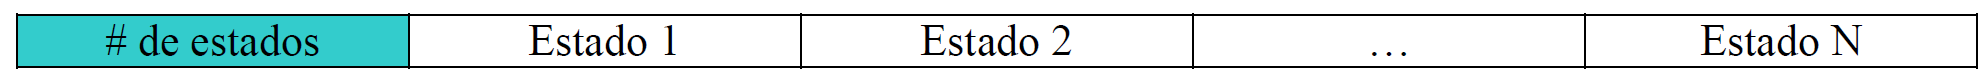
\includegraphics[width=0.9\textwidth]{images/img87.png}
	\label{figura87}
\end{figure}

Cada estado, a su vez, es un conjunto de variables de salida y decisiones (condicionales – “if”s) con las
variables de entradas.



Por ejemplo, el estado 1 se codificaría de la siguiente manera:

\begin{figure}[h!]
	\centering
	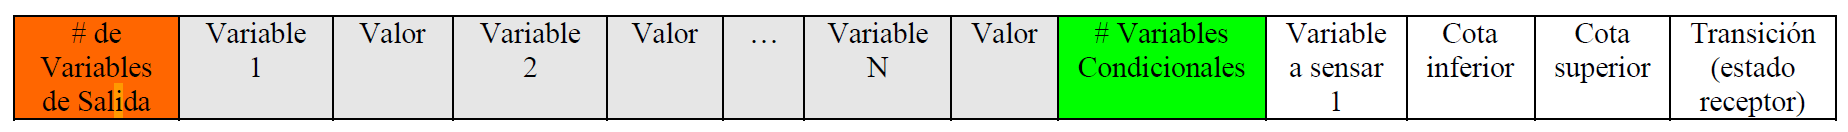
\includegraphics[width=0.9\textwidth]{images/img88.png}
	\label{figura88}
\end{figure}

...sigue...

\begin{figure}[h!]
	\centering
	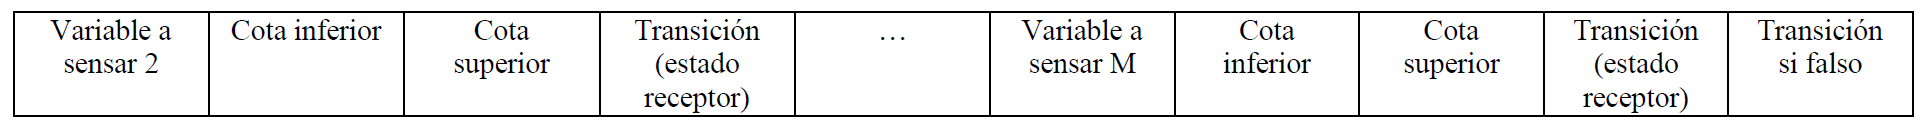
\includegraphics[width=0.9\textwidth]{images/img89.png}
	\label{figura89}
\end{figure}

\begin{ejemplo}
Codificar el estado (1) en: \\
$(1) Var5 = 7 \rightarrow (2)$
\end{ejemplo}

La solución es el binario de:

\begin{figure}[h!]

	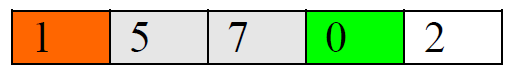
\includegraphics[width=0.3\textwidth]{images/img90.png}
	\label{figura90}
\end{figure}

Es decir: 

\begin{figure}[h!]
	
	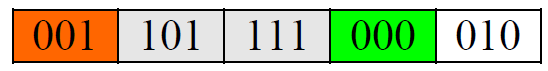
\includegraphics[width=0.3\textwidth]{images/img91.png}
	\label{figura91}
\end{figure}

\textbf{Ojo}: necesito una máquina que realmente evalúe este cromosoma y lo ejecute como una máquina de estados.

\begin{ejemplo}
	Codificar la máquina: \\
	$ (1) var1 = 3, var4 = 8 \rightarrow 10 < S3 < 25 ? (2) | (18)$
\end{ejemplo}

Solución: el binario de:

\begin{figure}[h!]
	
	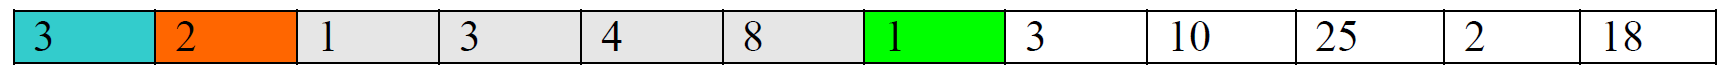
\includegraphics[width=0.9\textwidth]{images/img92.png}
	\label{figura92}
\end{figure}

\begin{ejemplo}
Codificar lo siguiente:
\end{ejemplo}


\begin{figure}[h!]
	
	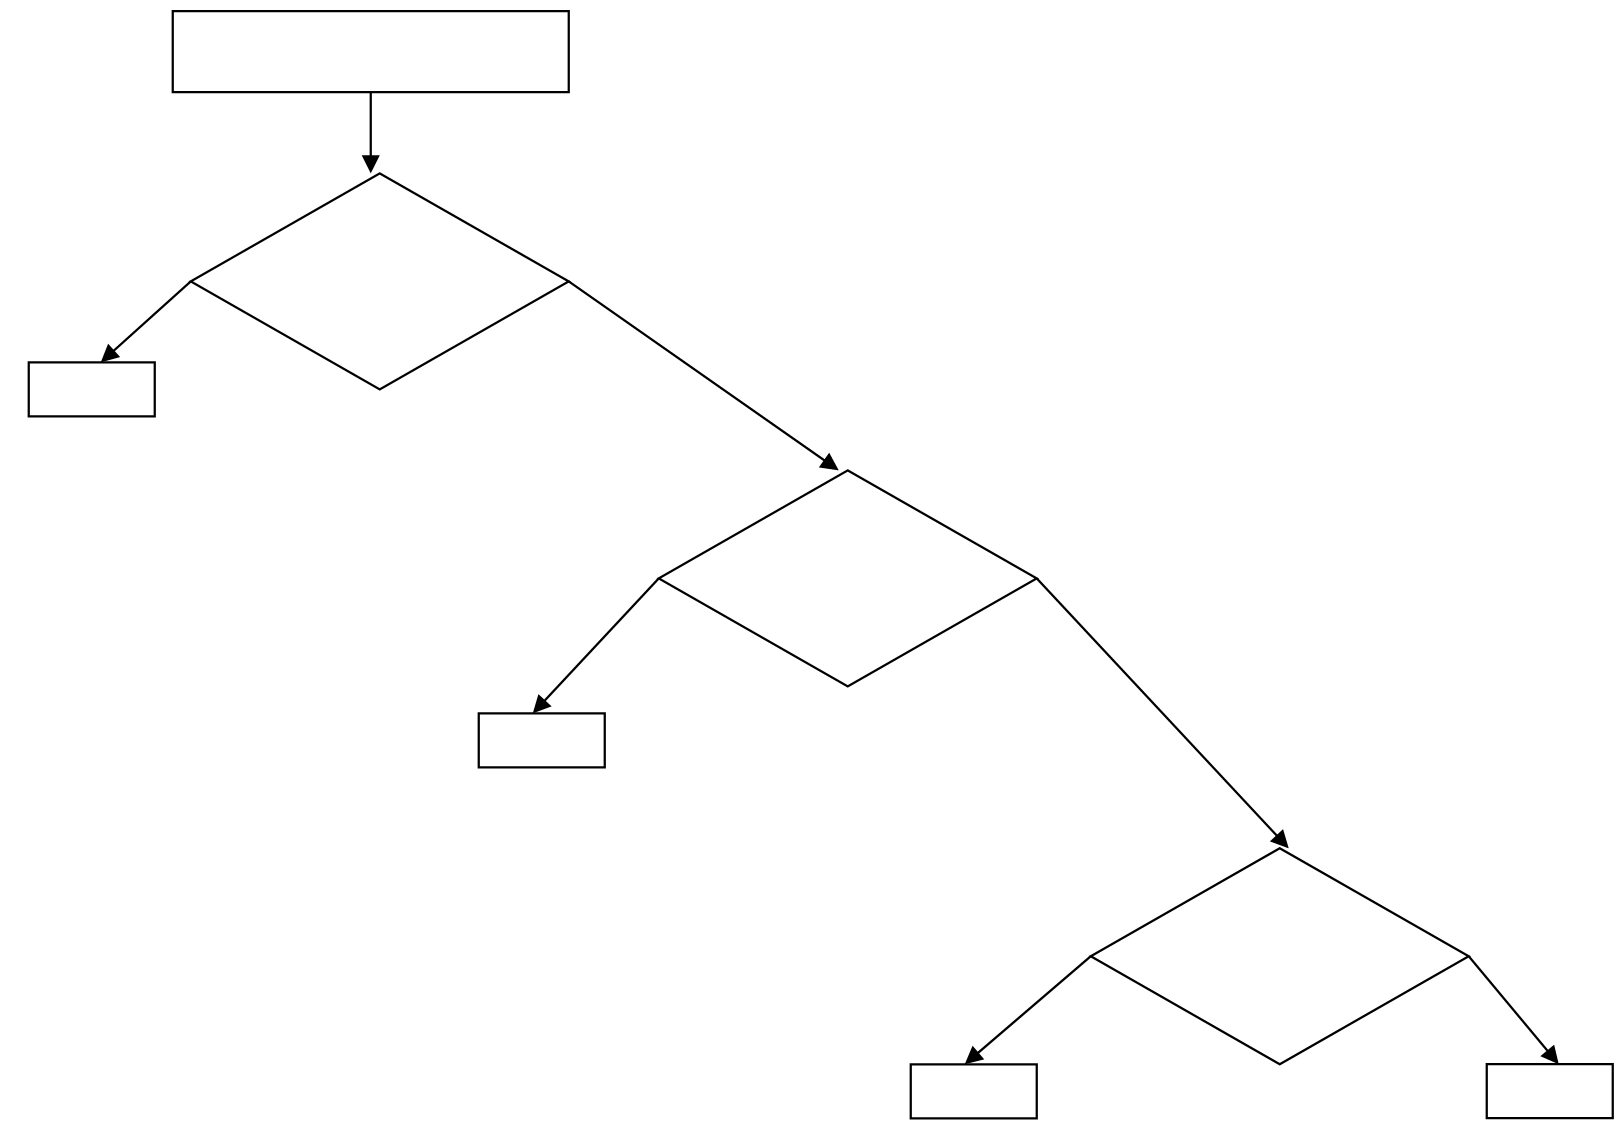
\includegraphics[width=0.8\textwidth]{images/img93.png}
	\label{figura93}
\end{figure}

 



\begin{nota}
LO IMPORTANTE ES QUE EL CROMOSOMA SE PUEDA EJECUTAR. Por ejemplo, si hay
condicionales de ambos lados no se puede con esta estructura.
\end{nota}

\begin{nota}
	Al hacer mutaciones o cruzamientos, hay que tener cuidado. Por ejemplo si se cruzan dos individuos
	de dos estados, y me da uno de un estado, habría que cortar el hijo para que la información posterior nada
	más tenga un estado. Igual si cambia a tres, añadir un estado. O cruzar condicionalmente... por ejemplo si
	cruzo el número de estados, podría tener que cruzar también la información de los estados etcétera.
\end{nota}


\begin{ejemplo}
	Codificar 
	\begin{equation}
	\begin{aligned}
		(1) M1 & = 0\ldotp 5; M2 = 0\ldotp3 \rightarrow 1 \ldotp 0 < S3 < 1\ldotp3 ? \\
		& T: (2) M1 = 0\ldotp1, M2 = 0\ldotp4  3\ldotp1 < S2 < 4\ldotp1 \\
		&\hspace{0.5cm} T: (2) \\
		&\hspace{0.5cm} F: 2\ldotp3 < S5 < 4 ? \\
		&\hspace{1cm}T: (3) M1 = 0\ldotp7, M2 = 0\ldotp7 \rightarrow 6 < S2 < 7\ldotp0 ? \\
		& \hspace{1.5cm} T: (3) \\ 
		& \hspace{1.5cm}F: 2\ldotp1 < S3 < 4\ldotp0 ? \\ 
		& \hspace{2cm}T: (3) \\
		& \hspace{2cm}F: (1) \\
		& \hspace{1cm}F: (2) \\ 
		& F: 3\ldotp1 < S1 < 4\ldotp7 ? \\
		& \hspace{0.5cm} T: (3) \\ 
		& \hspace{0.5cm}F: 1\ldotp1 < S2 < 1\ldotp2 ? \\
		& \hspace{1cm}T: (2) \\
		& \hspace{1cm}F: (1) \\ 
	\end{aligned}
	\end{equation}
\end{ejemplo}


\section{\underline{Utilización de algoritmos genéticos para organizar los comportamientos (arbitraje)}}

%imagen 
\begin{figure}[h!]
	\centering
	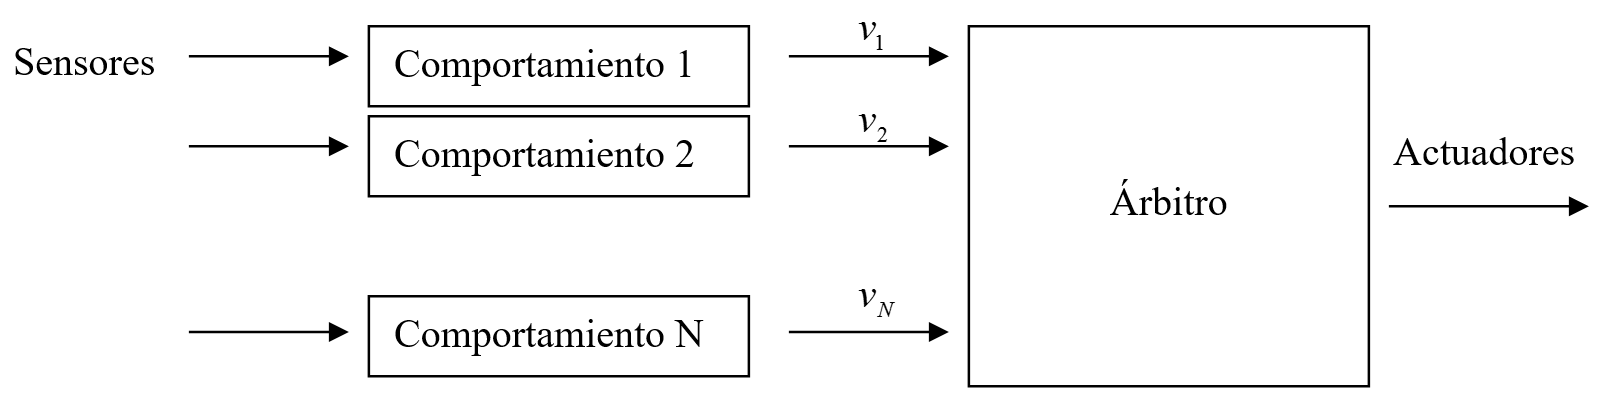
\includegraphics[width=0.9\textwidth]{images/img94.png}
	\label{figura94}
\end{figure}

Recuérdese que

$$c_f = \sum_{i=1}^{N} g_i \textbf{b}_i
 $$

donde $g_i$ son las constantes de ganancia y $\textbf{b}_i$ son los vectores de movimiento por los diferentes
comportamientos.

Además se tiene una \underline{función de desempeño global} que indica si el robot cumplió el objetivo.

\begin{itemize}
	\item[\textbullet]Una forma es encontrar las constantes g i con algoritmos genéticos, basándose en la función de
	desempeño global.
	\item[\textbullet]Otra forma de organizar es poniendo prioridades.
\end{itemize}

\subsection{Método de Utilidad Múltiple (Utility Manifold)}
Se quiere que el árbitro decida cuál de los comportamientos se debe activar.
Todos los comportamientos dan salidas siempre.
Cada comportamiento dirá su aplicabilidad, dependiendo de:

\begin{itemize}
		\item[\textbullet]los sensores internos
		\item[\textbullet]los sensores externos
\end{itemize}

Esto es un valor en (0,1)

1. Función de activación del comportamiento

$f_{H_i} (S_I, S_E , V)$

donde 

$S_I$ son los sensores internos (batería, odómetro, etc.)
$S_E$ son los sensores externos (sonares, infrarrojo, etc.) 
$V$ son variables de estado $x_1 ,..., x_r$

Se modela:

$f_{B_i}(S_E, S_I, x) = a_{i0} + a_{i1} S_E + a_{i2} S_I + a_{i3} x_i +  a_{i4} S_E^2 + a_{i5} S_I^2 + a_{i6} x_i^2 + a_{i7} S_E S_I + a_{i8} S_I x_i + a_{i9} S_E x_i ,$ para $i=1,\ldotp \ldotp \ldotp, n$ los $n$ comportamientos

Se quiere obtener $a_{ij}$ con algoritmos genéticos. 

Se definen: 

$ x_i = \begin{cases} b_{i1} + b_{i2} \; e^{-|b_{i3}|t_i}, \hspace{0.3cm} B_i \;$ est\'a activo $ \\
0,\hspace{0.3cm}   e.o.c.  
\end{cases} $	


Para cada comportamiento se tiene una función de activación. Se tienen diferentes individuos y, dentro
del cromosoma, se tiene:



\begin{figure}[h!]
\centering
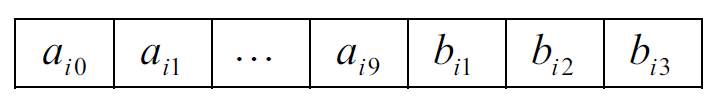
\includegraphics[width=0.6\textwidth]{images/img95.png}
\label{figura95}
\end{figure}
(en binario)

\begin{scaja}
	Resumen
	Los algoritmos genéticos se utilizan para introducir a los robots los comportamientos básicos. Esto NO corre
	en línea, es para “alambrar” los “instintos” al robot. 
\end{scaja}

\section{Planeación}

¿Cómo planear la ruta de un punto a otro? 

\begin{figure}[h!]
	\centering
	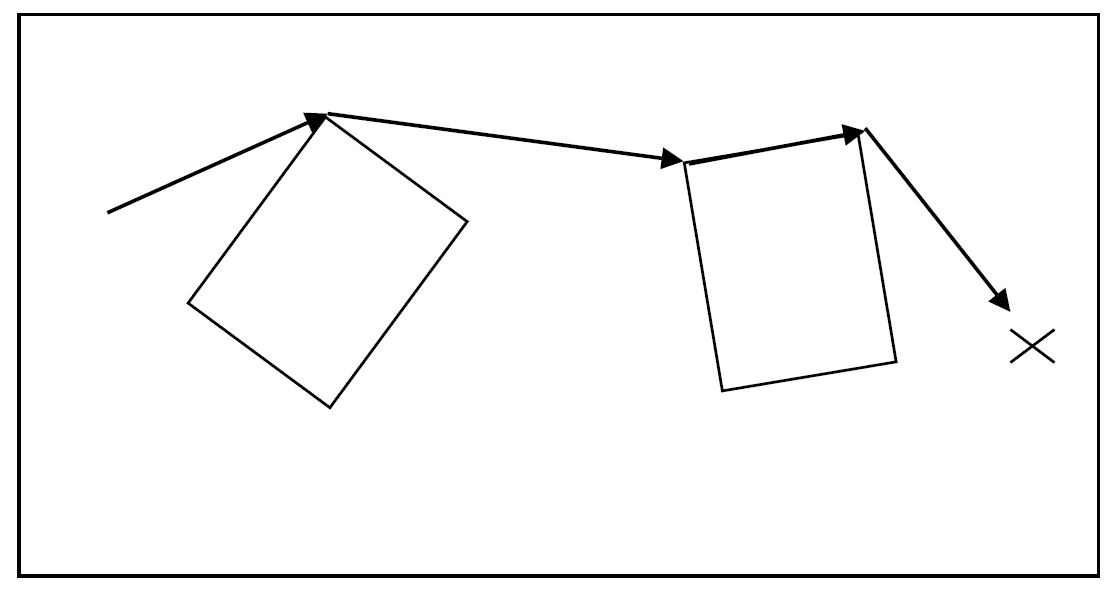
\includegraphics[width=0.6\textwidth]{images/img96.png}
	\label{figura96}
\end{figure}
(en binario)

Se quisiera encontrar camino más rápido.

Supóngase que se tiene un campo potencial y un obstáculo
¿Cómo se podría ajustar los campos potenciales?:

\begin{figure}[h!]
	\centering
	\includegraphics[width=0.6\textwidth]{images/img97.png}
	\label{figura97}
\end{figure}


Una idea podría ser tratar de encontrar \textit{varios} caminos por campos potenciales, dependiendo de un cierto
ángulo de desvío $\theta$.

Esto genera un árbol de opciones (caminos) que es muy costoso recorrer con \underline{fuerza bruta}. ¿Cómo recorremos
este árbol para que sea inteligente?

El objetivo es encontrar una mejor ruta para recorrerla. 

\subsection{Búsqueda de la mejor ruta}

El problema de búsqueda se puede formular como sigue:
 
\begin{scaja}
	Dado
	
	$x_0$ un punto inicial (o nodo)
	$x_f$ un punto objetivo (o nodo)
	un grafo con pesos (red topológica)
	
	se quiere encontrar una ruta óptima que llegue al punto objetivo desde el punto inicial y recorrerla.

\end{scaja} 

\begin{ejemplo}
	
Observe la siguiente imagen 

\end{ejemplo}

\begin{figure}[h!]
	\centering
	\includegraphics[width=0.6\textwidth]{images/img98.png}
	\label{figura98}
\end{figure}

\textbf{Depth-first}

Funciona para árboles

Es necesario convertir la red en árbol. Se ponen únicamente los caminos únicos (no recursivos).
Se ponen los pesos acumulados en cada nivel

Este approach se vuelve gigantesco, por lo que es necesario hacer un approach inteligente:

$\bullet$	Se va a realizar la búsqueda recorriendo el árbol por preorden hasta que sea nulo (en cuyo caso se
saca de la lista y se mete otro hijo del padre) o sea el objetivo.

S \\
A | S \\
B | A | S \\
C | B | A | S \\
E | B | A | S \\
D | E | B | A | S \\
F | E | B | A | S \\
G | F | E | B | A | S \\ 

Aquí ya se encontró el destino por lo que se encontró un camino de nodos. Ésta es la forma de encontrar un
camino.

La aplicación es:

\begin{enumerate}[1.]
	\item El planeador encuentra los nodos del grafo que hay que visitar	
	\item Cada uno se convierte en un punto de atracción sucesivo en el algoritmo de campos potenciales	
\end{enumerate}



\textbf{Hill Climbing}

Tiene una función heurística.
Generalmente la función del costo (o peso) al nodo más la distancia remanente al destino

$f(d(q_j, q_F), w_{ij})$

Es el costo de pasar de un nodo a otro más (por ejemplo) la distancia euclideana en R 3 del punto físico
asociado al nodo y el punto físico asociado al destino.

\textbf{Breadth-Search}

Se va guardando en una lista ligada
En cada iteración se van cargando los hijos de cada uno de los nodos de cada nivel.

\textbf{Planeación usando espacio-estado}

Reglas nombre {
	Precondiciones
	$\rightarrow$
	Operadores
	Lista de Borrado
	Lista Aditiva
}


\textit{Por ejemplo: Ponerse los zapatos:}


Regla Colocar$\_$Calcetin$\_$Derecho
Precondiciones

Colocar Zapato Derecho (comando) \\

Pie derecho está desnudo

Calcetín está disponible

$\rightarrow$

Operador

Poner$\_$Calcetin$\_$PieDerecho

Lista de Borrado

Calcetín está disponible

Pie derecho está desnudo


Regla Colocar$\_$Zapato$\_$Derecho \{
	Precondiciones
	
	No hay pie derecho desnudo
	
	Colocar Zapato Derecho (comando)
	
	Zapato derecho disponible
	
	$\rightarrow$
	
	Operador
	
	Poner zapato derecho
	
	Lista de borrado
	
	Zapato derecho disponible
	
	Colocar zapato derecho
\}



Se pueden organizar jerárquicamente:

Inicio

a) Colocar$\_$Calcetin$\_$derecho \\
a. Colocar$\_$zapato$\_$derecho \\
i. Colocar$\_$calcetin$\_$izquierdo \\
ii. Colocar$\_$zapato$\_$izquierdo \\

b. Colocar$\_$calcetin$\_$izquierdo \\
i. Colocar$\_$zapato$\_$izquierdo \\
1. Colocar$\_$zapato$\_$derecho \\
ii. Colocar zapato derecho \\
1. Colocar zapato$\_$izquierdo \\

b) Colocar$\_$Calcetin$\_$izquierdo\\
a. Colocar zapato izquierdo\\
i. Colocar calcetín derecho\\
ii. Colocar zapato derecho\\

b. Colocar calcetín derecho\\
i. Colocar zapato derecho\\
1. Colocar zapato izquierdo\\
ii. Colocar zapato izquierdo\\

1. Colocar zapato derecho\\


¿Por cuál camino irnos?
Debemos ponerle pesos y después trabajarlo con un algoritmo de búsqueda.


\begin{ejemplo}
	Bloques
	
	B	A	C	E	D
	Se quiere tener una representación espacio-estado con los operadores.
	
	B	D	C 	E	A
	
	
\end{ejemplo}

Operadores:


Goto(x,y,z) \hspace{0.5cm} Ir a (x,y,z) \\
Pickup(w) \hspace{0.5cm}Recoger w de la mesa \\
Putdown(w) \hspace{0.5cm}Soltar w en la mesa \\
Stack(u,v) \hspace{0.5cm}Poner el u encima del v \\
Unstack(u,v) \hspace{0.5cm} Quita el bloque u del v (y se lo queda en la mano)


La representación del estado del mundo:


Location(w,x,y,z) \hspace{0.5cm}  el bloque w está en las  coordenadas x,y,z \\
On(x,y) \hspace{0.5cm} el bloque x está encima de y \\
Clear(x) \hspace{0.5cm} no hay algo encima de x \\
Gripping(x) \hspace{0.5cm} el brazo del robot tiene el bloque x \\ (\textit{gripping(void)} es que no tiene algo) \\
OnTable(w) \hspace{0.5cm} el bloque w está en la mesa


A partir de esto se deduce que

$$\forall x (CLEAR(x)) \Rightarrow \neg \exists y (on(y,x)))$$
$$\forall x (GRIPPING (void) \Leftrightarrow \neg GRIPPING (x)$$
$$\forall y \forall x (ONTABLE (y) \Rightarrow \neg ON (y , x ))$$


Estado 1

	OnTable(A)\\
	OnTable(C)\\
	OnTable(D)\\
	On(B,A)\\
	On(E,D)\\
	Gripping(void) \\
	Clear(B) \\
	Clear(C) \\ 
	Clear(E)\\ 


Regla Pickup(x) \{
	Precondiciones \\
	Clear(x) \\
	OnTable(x) \\
	Gripping(void) \\
$\rightarrow$
	Lista de adición \\
	Gripping(x) \\ 
	Lista de borrado \\
	OnTable(x) \\
	Gripping(void) \\
\}


Observación: esto genera una \textit{notación de predicados}
 
$$ \forall x (PICKUP (x) \Rightarrow GRIPPING (x)) \leftarrow (GRIPPING (void) \textasciicircum CLEAR (x) \textasciicircum ONTABLE (x))
$$

Regla PutDown(x) \{ \\
	Precondiciones \\
	Gripping(x) \\
	$\rightarrow$
	Lista Adición \\
	Gripping(void) \\
	OnTable(x) \\
	Lista de Borrado \\
	Gripping(x) \\
\}

Regla Stack(x,y) \{ \\
	Precondiciones \\
	Gripping(x) \\
	Clear(y) \\
	$\rightarrow$ 
	Lista de adición \\
	Gripping(void) \\
	On(x,y) \\
	Lista de Borrado \\
	Gripping(x) \\
	Clear(y) \\
\}

Árbol de Estados

B A
C E
D


1) B
A E
C D

2)


A E
C D


Etcétera (todas las posibilidades)

\underline{Tercera evaluación}

Comportamiento de potenciales
Comportamiento de máquinas de estado
Árbitro


(con variables de aplicabilidad entre 0 y 1)



\textbf{Máquina de Inferencia}


Hechos + Reglas $\rightarrow$ Máquinas de Inferencia $\rightarrow$ Agenda
Los hechos activan reglas. Las reglas pueden generar otros hechos que, a su vez, pueden activar nuevas
reglas.

Por ejemplo esto puede evitar que en 100000 if’s anidados se tenga que ejecutar el último.
En lugar de que las reglas busquen los hechos que los activan, es al revés (puesto que los hechos
generalmente no cambian).


Las reglas producen hechos NUEVOS.

El sistema \textbf{CLIPS} es un lenguaje de programación orientado a plantillas que permite definir sistemas
expertos. Tiene una máquina de inferencia con encadenamiento hacia delante para eficiencia.
Permite definir hechos, reglas, etc.


\section{Lenguaje Natural}

La idea es hablarle a un robot en lenguaje cotidiano y que nos “entienda”. Entender es hacer un análisis
semántico para obtener un significado y transformarlo en una acci
ón.

Lo que yo le dije, que lo haga.

La definición operacional de \textbf{entender} es que el sistema realice las acciones que el usuario le pide.
Entender algo es transformar lo que se pide en una \textbf{representación}, la cual ha sido escogida para que
corresponda a un conjunto de acciones disponibles que pueden ser ejecutadas.


\begin{enumerate}[1.]
	\item Señal de entrada \\
	Puede ser voz, imagen o combinación de ambas (o cualquier otra forma de entrada, por teclado).
	Voz: por medio de un micrófono que transforma una señal acústica en una señal eléctrica.
	Es necesario aplicar técnicas de procesamiento digital de señales para obtener las características de
	esa señal acústica.
	Existen algoritmos (como el de cuantización vectorial y sus variantes) para procesar e identificar las
	palabras.
	
	\item Las palabras de entrada son revisadas para ver si ellas están agrupadas de acuerdo con reglas
	gramaticales, significando que ellas forman oraciones gramaticalmente correctas.
	
	\item El significado de cada palabra y de la oración es asignado.
	Este paso es el más difícil de los tres.
	
\end{enumerate}



\textit{Dependencia Conceptual}

\underline{Primitivas Conceptuales}

La representación de varias acciones es la misma.
Por ejemplo: “Juan dio el libro a Pedro”, “Juan prestó el libro a Pedro”, “Juan regaló el libro a Pedro”,
significan cosas diferentes, pero la acción de transferir el libro de una persona a otra es la misma.

Cada primitiva tiene:

\begin{enumerate}[a)]
	\item Un actor (realiza el acto)
	\item Un acto (realizado por el actor y hecho hacia un objeto)
	\item Un objeto (ente sobre el que es realizada la acción)
	\item Una dirección (en la cual el acto es realizado)
	\item Un estado (en el cual el objeto se encuentra)
\end{enumerate}

Las primitivas son:

\textbf{PTRANS} \hspace{0.5cm}
Es la transferencia física de un objeto. 

\hspace{2cm}
(PTRANS (Actor NIL) (Objeto NIL) (FROM NIL) (TO NIL) )

Por ejemplo

“Robot, lleva las flores al patio”
Se representaría como:

(PTRANS (Actor Robot) (Objeto flores) (From Posicion$\_$flores) (To Patio))
“Robot, ve a la cocina”
(PTRANS (Actor Robot) (Objeto Robot) (From Posicion$\_$robot) (To Cocina))

\textbf{Notar que el verbo indica qué primitiva utilizar}

MTRANS es la transferencia de información mental.
Roberto le dijo a Susana que era bonita
(MTRANS (ACTOR Roberto) (OBJETO “que Susana es bonita”) (FROM cerebro$\_$roberto) (TO
cerebro$\_$susana)
INGEST es la ingestión de un objeto por un animal, actor o ente
Juan toma leche
(INGEST (ACTOR Juan) (OBJECT Leche) (FROM NIL) (TO Boca$\_$Juan))
PROPEL es la aplicación de fuerza física a un objeto
María mató a una araña aventándole un zapato
(PROPEL (ACTOR María) (OBJECT Zapato) (FROM Brazo$\_$Maria) (TO Araña))
Observar: para matar a la araña con el PROPEL, primero tuvo que mover el brazo.
MOVE es el movimiento de una parte del cuerpo



Voz $\rightarrow$ Lenguaje natural de entrada y salida $\rightarrow$ PRIMITIVAS (Dependencia Conceptual) $\rightarrow$ Planeador de
acciones $\rightarrow$ Planeador de Rutas $\rightarrow$ Ambiente Virtual / Realidad

\begin{figure}[h!]
	\centering
	\includegraphics[width=0.6\textwidth]{images/img99.png}
	\label{figura99}
\end{figure}



\textbf{Proyecto Final}

1) \begin{enumerate}
	\item [1.] Red topológica con nodos
	\item [2.] Encontrar y ejecutar la mejor ruta
	\item [3.] 6 cubos en un array de 2x3
	
\end{enumerate}

2) Encontrar y ejecutar la mejor ruta
3) 6 cubos en un array de 2x3

A F | \\
B E | \\
C D | \\
Cuarto 1  cuarto 2 
\\

Poder ejecutar sentencias tipo “lleva A al cuarto 2”
(por ejemplo el A no se puede agarrar, hay que quitar C y B y ponerlos en otro lado)

Con CLIPS
Podemos poner nodos topológicos.


\section{Creación de Mapas}

La idea básica es crear un modelo del medio ambiente (una red topológica), basándose en la información en
los sensores.
Detectar con los sensores los puntos que delimitan el “espacio libre” (es decir, por donde puede navegar el
robot).

\subsection{Diagramas de Voronoi}

La idea es encontrar el diagrama de Voronoi de los puntos y entones el robot puede caminar sobre las líneas.

Considérese un punto $(x,y) \in C$ (el espacio libre). Los puntos bases de $(x,y)$ son los puntos $(x',y')$ más
cercanos en el espacio ocupado $\bar{C}$ . El diagrama de Voronoi es el conjunto de puntos en el espacio libre que
tiene cuando menos dos puntos bases diferentes a la misma distancia.


\textbf{Puntos Críticos}

Los puntos críticos $(x,y)$ son puntos en el diagrama de Voronoi tales que minimizan un margen local.
Existe $\varepsilon > 0$  tal que el margen de todos los puntos en la bola abierta de $(x,y)$ no es menor.


\textbf{Líneas críticas}

Son obtenidas conectando cada punto crítico con sus puntos base. Las líneas críticas particionan el espacio
libre en regiones disjuntas.

\subsection{Cuantización Vectorial}

Hacer clustering sobre el espacio libre.

\textbf{Clustering:}

Considérense $m$ vectores, $v_i = (x_i , y_i).$

\begin{enumerate}[1.]
	\item Encontrar un centroide $c_1 = \dfrac{1}{m} \sum_{j=1}^{m} v_j$
	
	\item Generar dos centroides nuevos a partir del centroide $C_i$ anterior
	$$c_{i+1} = c_i + \varepsilon_1$$
	$$C_{i+2} = C_i \varepsilon_2$$
	Donde $\varepsilon_k = 1 + \delta_k$, con $\delta_k$ pequeño en magnitud absoluta
	\item Agrupar los vectores en dos grupos de acuerdo al centroide más cercano.
	
	$$d_T = d(v_j , c_{i+r})    r=1,2$$
	
	\begin{center}
		Asignar a los grupos:
	\end{center}
	$$v_j \in G_{i+1}\Leftrightarrow d_1 < d_2$$
	$$v_j \in G_{i+2}\Leftrightarrow d_1 \leq d_2$$
	\begin{figure}[h!]
		\centering
		\includegraphics[width=0.4\textwidth]{images/img100.png}
		\label{figura100}
	\end{figure}

\end{enumerate}
	\break



\textbf{Localización del Robot}


Si el odómetro fuera perfecto, se puede saber siempre en dónde se encuentra el robot. Sin embargo, en la
realidad no son exactos y no se sabe.
Se puede utilizar la visión para localizar puntos de referencia predefinidos.
Para hacer esto, se necesita que el sistema de visión sea invariante al tamaño y a transformaciones
(rotaciones).
Ya sea con un sistema de visión o de localización, se puede hacer triangulación.
Si se tienen varias marcas, suponiendo que se pueden encontrar las distancias a las marcas, se puede trazar un
círculo de radio la distancia.
Se establece entonces:

$$(z-z_i)^2 + (z-z_i)^2 + (z-z_i)^2 =d_{i}^2 \hspace{0.5cm} ,   \forall_i$$

El sistema de ecuaciones me determina $(x , y , z)$, es decir, la posición del robot.

Esto podría funcionar pero los sensores tienen errores y por lo tanto nunca se intersecan los círculos.
Por lo tanto, la localización del robot es probabilística

4. Si $D_{g}^t - D_{g}^{t-r} > \epsilon $ entonces recalcular los centroides

$$c_{i+r} = \dfrac{1}{m_{{G}_{i+r}}} = \sum_{j=1}^{m_{{G}_{i+r}}} v_j, \;\;  r=1,2$$

donde $D_{g}^t = \displaystyle\sum_{j=1}^{t} min (d_1 (j),d_2 (j))$ y $t$ es la iteración

Si es mayor, ir al punto 3.
Si es menor:

Repetir 2 hasta que se tenga el número de centroides deseado.

\subsection{Cadenas de Markov y Modelos Ocultos de Cadenas de Markov}

Una cadena de Markov es como una máquina de estado en la que las transiciones son probabilísticas.

$$a_{ij} = P [pasar de i a j]$$

Los cambios de estado están indexados al tiempo y se denominan $q_t$.

Un proceso estocástico es un \textbf{proceso markoviano de primer orden} si la probabilidad de que la cadena de
Markov se encuentre en un determinado estado j es:

$$P[q_t = j \;| \; q_{t-1} = i_1, \; q_{t-2} = i_2,\ldots, q_0 = i_t] = P[q_t = j|q_{t-1} = i]$$

Se tiene:

$$a_{ij} \; > 0 \forall i, j$$
$$\sum_{j=1}^{N} a_{ij} = 1 \forall i$$

<falta una clase aquí>


\begin{caja}
\textbf{Problema 1}

\begin{math}
O=(O_1, O_2, \ldots , O_N)\\ 
\lambda = (A,B,\Pi) \\
P(O|\lambda)\\
\end{math}


Con lo visto anteriormente, son aproximadamente \((2T-1)N^T+N^T-1\) operaciones. Por ejemplo, con 5
estados y \(100\) observaciones, esto es aproximadamente \(10^{72}\) operaciones. Por tanto, necesitamos obtener
algún procedimiento más eficiente.

\end{caja}

\textbf{Procedimiento hacia delante}

$\alpha_t (i) = P(O_1, O_2, \ldots, \; O_t, q_t = i|\lambda) $

Es la probabilidad de observar la secuencia parcial $O_1, O_2, \ldots, O_t$ y el estado $i$ en el tiempo $t$.

Esta probabilidad se puede encontrar de manera inductiva:


\begin{enumerate}[1.]
	\item Inicialización
	
	$\alpha_1 (i) = \Pi_i b_i (O_1), 1\leq i \leq N$
	
	$O_i$ es la observación al tiempo $i$. 
	
	Por ejemplo, se puede tener: $O_1=v_4$ que es una mesa.
	Las probabilidades son fijas pero las observaciones están cambiando respecto al tiempo.
	
	\item Inducción
	
	$\alpha_{t+1} (j) = \left[ \displaystyle \sum_{i=1}^{N} \alpha_t (i) a_{ij}\right] b_j (O_{t+1}) \; 1 \leq t \leq T -1, \; 1\leq j \leq N $
	
	 La probabilidad depende de la probabilidad anterior, las probabilidades de transición y la probabilidad de
	 la observación en el estado $j$.
	
	
	\item Término
	
	$P(O| \lambda) = \displaystyle \sum_{i=1}^{N} \alpha_T (i) = \displaystyle \sum_{k=1}^{N} P(O_1, O_2, \ldots, \; O_t, q_t = i|\lambda)$
	
	Para calcular $\alpha_t (j) 1 \leq t \leq T, \; 1\leq j \leq N$ se requieren $N^2 T$ cálculos (en lugar de $2TN^T$)
	
	
\end{enumerate}


\begin{caja}
	\textbf{Problema 2}
	
	
	Encontrar la mejor secuencia de estados \( q = (q_1, q_2 , \ldots, q_T)\)dada la secuencia de observaciones \( O = (O_1, O_2, \ldots, O_T)\)
	En términos del robot: dado lo que vio, en dónde se estuvo moviendo.
	
\end{caja}

\textbf{Diagrama de Trellis}

Diagrama de Trellis

Dado una máquina de estados con transiciones:

\begin{figure}[h!]
	\centering
	\includegraphics[width=0.9\textwidth]{images/img101.png}
	\label{figura101}
\end{figure}

Para cada estado hay una serie de caminos, hay que encontrar el mejor camino. Sin embargo, para cada
tiempo, la búsqueda crece en forma exponencial (el número de caminos crece).

Hay que hacerlo con el \textbf{Algoritmo de Viterbi}, que va eliminando todos los caminos menos los más
probables.

\section{Algoritmo de Viterbi}


Sea $\delta_t (i)$la mejor ruta en el tiempo $t$ que toma en cuenta las primeras $t$ observaciones y termina en el estado
$i$.

$\delta_t (i) = \underset{q_1, \ldots, q_{t1}}{max} P[q_1 q_2 \ldots q_{t-1}, q_t = i, O_1 , O_2, \ldots, O_t | \lambda]$

\begin{enumerate}
	\item [1)] Inicialización
	
	$\delta_i (i) = \pi_i b_i (O_1)$ para  toda $i$
	
	\item[2)]Recursión
	
	$\delta_t (j) = \lgroup \underset{1\leq i\leq N}{max} \left [ \delta_{t-1} (i) a_{ij }\right] \rgroup b_j (O_t)$
	
	$ 2\leq t \leq N , 1 \leq j \leq N$
	
	$\Psi_t (j) = \underset{1\leq i\leq N}{arg max} \left [ \delta_{t-1 (i) a_{ij}}\right] $ (es decir, los nodos que conforman la ruta)
	
	\item[3)]Término
	
	$p^* = \underset{1\leq i\leq N}{max} \left[ \delta_T (i) \right]$
	
	$q_{{T}}^* = \underset{1\leq i\leq N}{arg max} \left[ \delta_T (i) \right]$
	
	
	\item[4)]Ruta
	
	
	La ruta se obtiene:
	
	$q_{t}^* = \Psi_{t+1} (q_{t+1}^*), \enspace t = T-1, \: T-2, \ldots, 1 
	$
	
\end{enumerate}

\begin{caja}
	\textbf{Problema 3}
	\\
	\textbf{Estimación de Parámetros} 
	\\
	
	
	Se quiere encontrar $\lambda = (A,B,\pi) $ que satisfaga un cierto criterio de optimalidad. \\
		
	Modelo inicial $\rightarrow$ (de datos de entrenamiento) Segmentación secuencia de estados $\rightarrow$  Reestimación del
	modelo $\rightarrow$ Convergencia del modelo? Si sí, regresar a segmentación, si no, dar parámetros del modelo. \\
	
	$b_j (k)$ es el número de observaciones con el símbolo $k$ en el estado $j$ dividido por el número de
	observaciones en el estado $j$. \\
	
	
	
	$a_{ij}$ es el número de transiciones del estado $i$ al estado $j$ dividido por el número de transiciones de $i$ a cualquier
	estado.
	$\pi_i$ es el número de veces que se empezó en el estado $i$ dividido entre el número de veces de entrenamientos.
\end{caja}




